\documentclass[12pt,a4paper]{article}

% ------------------------------------------------
% PAQUETES
% ------------------------------------------------
\usepackage[utf8]{inputenc}
\usepackage[T1]{fontenc}
\usepackage[spanish,es-tabla]{babel}

\usepackage{amsmath}
\usepackage{amssymb}
\usepackage{natbib}

\usepackage{algorithm}
\usepackage{algorithmic}

\usepackage{float}
\usepackage{booktabs}
\usepackage{array}
\newcolumntype{L}[1]{>{\raggedright\arraybackslash}p{#1}}
\usepackage{url}
\usepackage[hidelinks]{hyperref}

\floatname{algorithm}{Algoritmo}
\renewcommand{\algorithmicrequire}{\textbf{Entrada:}}
\renewcommand{\algorithmicensure}{\textbf{Salida:}}
\renewcommand{\algorithmiccomment}[1]{\hfill$\triangleright$~#1}

\makeatletter
\newcommand{\PARFOR}[2]{\STATE \textbf{for} #1 \textbf{pardo} \COMMENT{#2}\begin{ALC@g}}
\newcommand{\ENDPARFOR}{\end{ALC@g}\STATE \textbf{end for}}
\newcommand{\PROCEDURE}[2]{\STATE \textbf{procedure} \textsc{#1}(#2)\begin{ALC@g}}
\newcommand{\ENDPROCEDURE}{\end{ALC@g}\STATE \textbf{end procedure}}
\newcommand{\FUNCTION}[2]{\STATE \textbf{function} \textsc{#1}(#2)\begin{ALC@g}}
\newcommand{\ENDFUNCTION}{\end{ALC@g}\STATE \textbf{end function}}
\makeatother


\usepackage{geometry}
\usepackage{graphicx}
\geometry{margin=2.5cm}

% ------------------------------------------------
% DOCUMENTO
% ------------------------------------------------
\begin{document}
\begin{titlepage}
    \centering

    
\includegraphics[width=0.32\textwidth]{utec_logo.png}

    \vspace{1.5cm}

    {\Large
    \textbf{Universidad de Ingeniería y Tecnología -- UTEC}
    \par}

    \vspace{1.8cm}

    {\LARGE
    \textbf{Proyecto final}
    \par}

    \vspace{0.5cm}

    {\Large
    CS4052 – Computación Paralela y Distribuida
    \par}

    \vspace{1.2cm}

    {\Large
    \textbf{Problema del Agente Viajero (TSP)}
    \par}

    \vfill

    {\large
    \textbf{Integrantes}\\[0.3cm]
    Melanie Alexia Cortez Rojas - 100\% \\
    Sergio Sebastian Lezama Orihuela - 100\% \\
    Federico Iribar Casanova - 100\% 
    \par}

    \vspace{1.5cm}

    {\large
    \textbf{Docente}\\
    Jose Antonio Fiestas Iquira 
    \par}

    \vspace{1.2cm}

    {\large
    \textbf{Repositorio}\\
    \url{https://github.com/SergioSLO/tsp-bnb-openmp}
    \par}

    \vspace{1.2cm}

    {\large 2026\par}

\end{titlepage}



\vspace{0.5cm}

\section{Introducción}

El proyecto elegido es el Problema del Agente Viajero (TSP, por sus siglas en inglés). Dadas $n$ ciudades y el costo de viajar entre cada par de ellas, el objetivo es encontrar
el recorrido de menor costo total que visite cada ciudad exactamente una vez y regrese a la ciudad de partida. Formalmente, dado un grafo completo $G=(V,E)$ con $|V|=n$ y una función de costo $c: E \rightarrow \mathbb{R}_{\geq 0}$, se busca un ciclo hamiltoniano de costo mínimo \citep{applegate2006tsp}.

El TSP es un problema NP-difícil \citep{garey1979computers}, por lo que no se conoce ningún algoritmo que lo resuelva de forma exacta en tiempo polinomial. En su versión simétrica existen $\frac{(n-1)!}{2}$ rutas posibles, de modo que evaluarlas todas se
vuelve impracticable incluso para instancias pequeñas: con solo 20 ciudades hay aproximadamente $6 \times 10^{16}$ recorridos distintos.

Entre los distintos enfoques propuestos para resolver el TSP, en este proyecto se utiliza el método de \textit{Branch and Bound}, aplicado al problema por primera vez por \citet{little1963algorithm}. Se trata de un método exacto que organiza las rutas parciales en un árbol de búsqueda y descarta aquellas ramas cuya cota inferior indica que no pueden mejorar la mejor solución encontrada hasta el momento. Este método resulta adecuado para la paralelización, ya que las distintas ramas del árbol pueden explorarse de forma prácticamente independiente y distribuirse entre varios procesadores, que solo necesitan compartir el costo de la mejor solución hallada \citep{grama2003introduction}.

Entre las dos aplicaciones propuestas en el enunciado, se eligió encontrar la ruta aérea más corta entre 10 puntos geográficos ubicados en distintos países y comparar los resultados con 20 puntos, en lugar de utilizar el conjunto de datos VLSI \citep{cook_vlsi}. Debido al crecimiento factorial del espacio de búsqueda, \textit{Branch and Bound} deja de ser práctico a partir de aproximadamente 20 a 25 ciudades, mientras que incluso la instancia VLSI más pequeña (\texttt{xqf131}) cuenta con 131 puntos, lo que obligaría a recortarla de forma considerable y a perder la referencia a su óptimo publicado. Además, las instancias pequeñas permiten validar la correctitud del algoritmo: para $n=10$ existen $9!/2 = 181\,440$ rutas, que pueden evaluarse por fuerza bruta y compararse con el resultado obtenido. Trabajar con dos tamaños de problema, complementados con tamaños intermedios, permite también analizar la escalabilidad del algoritmo paralelo. Las distancias entre puntos se calculan sobre la superficie terrestre mediante la fórmula de haversine. Como extensión, en la Sección~\ref{sec:vlsi} también se resuelven instancias recortadas de \texttt{xqf131} de hasta 33 puntos, con una cota mejorada.

El algoritmo se implementó en C++ con OpenMP en tres versiones (secuencial, \texttt{parallel for} y tareas), más una cuarta con una cota mejorada, y se ejecutó en el clúster Khipu de la UTEC. La Sección~\ref{sec:impl} describe la implementación y la Sección~\ref{sec:resultados} presenta y analiza los resultados.

\section{Algoritmo secuencial}

El algoritmo utiliza el método de \textit{Branch and Bound} para encontrar la ruta de menor costo que permita visitar todas las ciudades exactamente una vez y regresar a la ciudad inicial.

La búsqueda genera diferentes rutas parciales. Para cada ruta se calcula una cota inferior (\textit{bound}) que permite determinar si la rama puede ser descartada. Si la cota es mayor o igual que el costo de la mejor solución encontrada hasta el momento, dicha rama no se continúa explorando.

El pseudocódigo se divide en tres partes independientes, cada una con sus entradas y salidas: la función \textsc{CalcularBound} (Algoritmo~\ref{alg:bound}), el procedimiento recursivo \textsc{Buscar} (Algoritmo~\ref{alg:buscar_sec}) y el programa principal \textsc{Main} (Algoritmo~\ref{alg:main_sec}). A la derecha de cada paso se anota su complejidad ($\triangleright$), de modo que el tiempo total y las métricas de la Sección~\ref{sec:paralelo} pueden leerse directamente del pseudocódigo. La matriz de distancias $D$ es de solo lectura una vez construida.

\begin{algorithm}[H]
\caption{\textsc{CalcularBound}: cota inferior de una ruta parcial}
\label{alg:bound}
\begin{algorithmic}[1]
    \REQUIRE $costo$ (costo de la ruta parcial), $visitada[0\dots n-1]$, $D[0\dots n-1][0\dots n-1]$
    \ENSURE $bound$, cota inferior del costo de cualquier ruta completa que extienda la ruta parcial
    \FUNCTION{CalcularBound}{$costo,\ visitada$}
        \STATE $bound \gets costo$ \COMMENT{$O(1)$}
        \FOR[$n$ iteraciones $\Rightarrow O(n^2)$ en total]{$i \gets 0$ \TO $n-1$}
            \IF[$O(1)$]{$visitada[i] = FALSE$}
                \STATE $min\_dist \gets \infty$ \COMMENT{$O(1)$}
                \FOR[$O(n)$]{$j \gets 0$ \TO $n-1$}
                    \IF[$O(1)$]{$i \neq j$ \AND $D[i][j] < min\_dist$}
                        \STATE $min\_dist \gets D[i][j]$
                    \ENDIF
                \ENDFOR
                \STATE $bound \gets bound + min\_dist$ \COMMENT{$O(1)$}
            \ENDIF
        \ENDFOR
        \RETURN $bound$
    \ENDFUNCTION
\end{algorithmic}
\end{algorithm}

\begin{algorithm}[H]
\caption{\textsc{Buscar}: exploración secuencial del árbol (Branch and Bound)}
\label{alg:buscar_sec}
\begin{algorithmic}[1]
    \REQUIRE $ciudad$ (última ciudad de la ruta parcial), $nivel$ (ciudades ya incluidas), $costo$ (costo acumulado); variables globales $D$, $visitada$, $ruta$, $mejor\_costo$, $mejor\_ruta$
    \ENSURE $mejor\_costo$ y $mejor\_ruta$ actualizados con la mejor ruta del subárbol
    \PROCEDURE{Buscar}{$ciudad,\ nivel,\ costo$}
        \IF[hoja: ruta completa]{$nivel = n$}
            \STATE $costo\_total \gets costo + D[ciudad][0]$ \COMMENT{$O(1)$}
            \IF[$O(1)$]{$costo\_total < mejor\_costo$}
                \STATE $mejor\_costo \gets costo\_total$ \COMMENT{$O(1)$}
                \STATE $mejor\_ruta \gets ruta$ \COMMENT{$O(n)$ copia}
            \ENDIF
            \RETURN
        \ENDIF
        \FOR[$n-nivel$ hijos]{$siguiente \gets 0$ \TO $n-1$}
            \IF[$O(1)$]{$visitada[siguiente] = FALSE$}
                \STATE $nuevo\_costo \gets costo + D[ciudad][siguiente]$ \COMMENT{$O(1)$}
                \STATE $bound \gets$ \textsc{CalcularBound}$(nuevo\_costo,\ visitada)$ \COMMENT{$O(n^2)$}
                \IF[poda, $O(1)$]{$bound < mejor\_costo$}
                    \STATE $visitada[siguiente] \gets TRUE$;\ $ruta[nivel] \gets siguiente$ \COMMENT{$O(1)$}
                    \STATE \textsc{Buscar}$(siguiente,\ nivel+1,\ nuevo\_costo)$ \COMMENT{subárbol}
                    \STATE $visitada[siguiente] \gets FALSE$ \COMMENT{$O(1)$ backtracking}
                \ENDIF
            \ENDIF
        \ENDFOR
    \ENDPROCEDURE
\end{algorithmic}
\end{algorithm}

\begin{algorithm}[H]
\caption{\textsc{Main} secuencial}
\label{alg:main_sec}
\begin{algorithmic}[1]
    \REQUIRE $n$; coordenadas geográficas $(lat_i, lon_i)$, $i = 0,\dots,n-1$
    \ENSURE $mejor\_costo$ (longitud del ciclo hamiltoniano mínimo) y $mejor\_ruta$
    \FOR[$O(n^2)$]{$i \gets 0$ \TO $n-1$}
        \FOR{$j \gets 0$ \TO $n-1$}
            \STATE $D[i][j] \gets \textsc{Haversine}(lat_i, lon_i, lat_j, lon_j)$ \COMMENT{$O(1)$}
        \ENDFOR
    \ENDFOR
    \STATE $mejor\_costo \gets \infty$;\ $mejor\_ruta \gets \emptyset$;\ $visitada[0\dots n-1] \gets FALSE$ \COMMENT{$O(n)$}
    \STATE $ruta[0] \gets 0$;\ $visitada[0] \gets TRUE$ \COMMENT{$O(1)$}
    \STATE \textsc{Buscar}$(0,\ 1,\ 0)$ \COMMENT{$O(n^2 (n-1)!)$ peor caso}
    \RETURN $mejor\_costo,\ mejor\_ruta$
\end{algorithmic}
\end{algorithm}

\subsection{Descripción}

El algoritmo comienza fijando la ciudad $0$ como ciudad inicial. La variable
$visitada$ permite controlar qué ciudades han sido incluidas en la ruta
actual.

En cada nivel del árbol de búsqueda, se recorren mediante un ciclo
\texttt{FOR} todas las ciudades que todavía no han sido visitadas. Para
cada una de ellas se calcula el nuevo costo de la ruta parcial y una cota
inferior.

Si la cota obtenida cumple

\[
bound < mejor\_costo,
\]

la rama continúa siendo explorada. En caso contrario, la rama se descarta,
ya que no puede producir una solución mejor que la encontrada actualmente.

Cuando se alcanza el nivel $n$, todas las ciudades han sido visitadas. En
ese momento se agrega el costo del regreso a la ciudad inicial y se compara
la ruta completa con la mejor solución almacenada.

La cota calculada por \textit{CalcularBound} es una cota inferior válida. Al
momento de calcularla, la ciudad $siguiente$ aún no está marcada como visitada,
por lo que la suma considera a $siguiente$ y a todas las ciudades pendientes.
Para completar la ruta, de cada una de estas ciudades debe salir exactamente una
arista: de $siguiente$ hacia la próxima ciudad, y así sucesivamente hasta la
última, que regresa a la ciudad $0$. El costo de cada una de esas aristas es al
menos el de la arista más barata que sale de su ciudad, por lo que $bound$ nunca
sobreestima el costo de la mejor ruta que extiende la ruta parcial. En
consecuencia, la rama que contiene la solución óptima nunca es descartada: si una
rama se poda porque $bound \geq mejor\_costo$, ya se cuenta con una solución de
costo igual o menor. Esto garantiza que el algoritmo es exacto.

\subsection{Complejidad secuencial}
\label{sec:compl_sec}

El algoritmo se ejecuta de manera recursiva, explorando los distintos caminos
posibles con el objetivo de encontrar la ruta de menor costo. Cada vez que se
completa un recorrido, este se compara con la mejor solución encontrada hasta ese
momento y, si presenta un costo menor, se actualiza dicha solución.

Al analizar el número de caminos que pueden generarse, el problema corresponde a
una enumeración combinatoria. Considerando que la ciudad inicial se encuentra
fijada, para la primera elección existen $n-1$ ciudades disponibles. Una vez
seleccionada una de ellas, quedan $n-2$ posibilidades para la siguiente posición,
luego $n-3$, y así sucesivamente hasta llegar a la última ciudad. Por lo tanto, el
número máximo de recorridos completos es
\[
(n-1)(n-2)(n-3)\cdots 2 \cdot 1 = (n-1)!.
\]
Este valor es el doble de las $\frac{(n-1)!}{2}$ rutas distintas mencionadas en la
introducción, ya que el algoritmo no aprovecha la simetría del problema: cada ruta
se explora en ambos sentidos (por ejemplo, $0 \to 1 \to 2 \to 3 \to 0$ y
$0 \to 3 \to 2 \to 1 \to 0$), aunque ambas tengan el mismo costo.

Sin embargo, la cota no se calcula solo en las rutas completas (las hojas del
árbol), sino en cada nodo generado, es decir, también en todas las rutas
parciales. El número total de nodos del árbol es
\[
\sum_{k=1}^{n-1} \frac{(n-1)!}{(n-1-k)!}
= (n-1)! \sum_{j=0}^{n-2} \frac{1}{j!}
\leq e \cdot (n-1)!,
\]
por lo que sigue siendo del orden de $O\left((n-1)!\right)$.

En cada uno de estos nodos, el algoritmo ejecuta la función
\textit{CalcularBound}, cuya implementación contiene dos ciclos anidados que
recorren las ciudades. Por esta razón, el cálculo de la cota inferior presenta una
complejidad de $O(n^2)$.

Al combinar el número de nodos con el costo de calcular el \textit{bound} en cada
uno, se obtiene, para el peor caso, una complejidad temporal de
\[
T_s(n) = O\left(n^2 \cdot (n-1)!\right).
\]
Como $n \cdot (n-1)! = n!$, esta expresión es equivalente a
\[
\boxed{T_s(n) = O(n \cdot n!)}.
\]

Esta corresponde a la complejidad del algoritmo secuencial en el peor caso. En la
práctica, \textit{Branch and Bound} puede presentar un tiempo de ejecución
considerablemente menor debido a la poda de ramas que no pueden producir una
solución mejor que la encontrada hasta ese momento. Sin embargo, en el peor caso,
cuando la poda resulta insuficiente, el algoritmo puede llegar a explorar una
cantidad factorial de caminos.




\section{Algoritmo Paralelo}
\label{sec:paralelo}

\subsection{Modelo PRAM y paradigma}

La versión paralela se diseña sobre el modelo \textbf{PRAM CRCW} (\textit{Concurrent Read Concurrent Write}) y se implementó en C++ con \textbf{OpenMP} (memoria compartida), que es el paradigma que corresponde a este modelo: todos los hilos leen la misma matriz de distancias y comparten la mejor solución, sin necesidad de enviar mensajes explícitos.
\begin{itemize}
    \item \textbf{Lectura concurrente (CR):} todos los procesadores leen simultáneamente la matriz $D$ (solo lectura) y el valor actual de $mejor\_costo$ para decidir la poda.
    \item \textbf{Escritura concurrente (CW) con prioridad mínima:} varios procesadores pueden llegar a una hoja a la vez e intentar actualizar la mejor solución. Se asume una escritura concurrente con prioridad (\textit{MIN-CRCW}): entre las escrituras simultáneas prevalece la de menor $costo\_total$, y el par $(mejor\_costo, mejor\_ruta)$ se escribe como una sola unidad, de modo que el costo y la ruta guardados siempre corresponden entre sí.
    \item \textbf{Estado privado:} los arreglos $visitada$ y $ruta$ describen la ruta parcial de \emph{una} rama. Si fueran globales, los procesadores que exploran ramas distintas dentro del mismo \textbf{pardo} los sobrescribirían entre sí (condición de carrera). Por ello, cada procesador trabaja sobre copias privadas $vis$ y $r$, que se pasan como parámetros a la llamada recursiva.
\end{itemize}

La estrategia es paralelismo de tareas sobre el árbol de búsqueda: el ciclo que elige la siguiente ciudad se convierte en un \textbf{pardo}, de manera que cada hijo del nodo actual es explorado por un procesador distinto. La función \textsc{CalcularBound} (Algoritmo~\ref{alg:bound}) no cambia: se ejecuta de forma secuencial dentro de cada procesador, porque su costo ($O(n^2)$, a lo más $400$ operaciones para $n=20$) es demasiado pequeño para justificar paralelismo de grano fino.

\begin{algorithm}[H]
\caption{\textsc{BuscarPar}: exploración paralela del árbol (PRAM CRCW)}
\label{alg:buscar_par}
\begin{algorithmic}[1]
    \REQUIRE $ciudad$, $nivel$, $costo$; copias privadas $r[0\dots n-1]$ (ruta parcial) y $vis[0\dots n-1]$; compartidas: $D$ (lectura), $mejor\_costo$, $mejor\_ruta$ (CR, MIN-CW)
    \ENSURE $(mejor\_costo, mejor\_ruta)$ actualizados con la mejor ruta del subárbol
    \PROCEDURE{BuscarPar}{$ciudad,\ nivel,\ costo,\ r,\ vis$}
        \IF[hoja: ruta completa]{$nivel = n$}
            \STATE $costo\_total \gets costo + D[ciudad][0]$ \COMMENT{$O(1)$}
            \IF[$O(1)$, CR]{$costo\_total < mejor\_costo$}
                \STATE $(mejor\_costo, mejor\_ruta) \gets (costo\_total, r)$ \COMMENT{$O(n)$, MIN-CW}
            \ENDIF
            \RETURN
        \ENDIF
        \PARFOR{$siguiente \gets 0$ \TO $n-1$}{$O(1)$; $n-nivel$ procesadores}
            \IF[$O(1)$]{$vis[siguiente] = FALSE$}
                \STATE $nuevo\_costo \gets costo + D[ciudad][siguiente]$ \COMMENT{$O(1)$}
                \STATE $bound \gets$ \textsc{CalcularBound}$(nuevo\_costo,\ vis)$ \COMMENT{$O(n^2)$ secuencial}
                \IF[poda, $O(1)$, CR]{$bound < mejor\_costo$}
                    \STATE $vis' \gets vis$;\ $r' \gets r$ \COMMENT{$O(n)$ copia privada}
                    \STATE $vis'[siguiente] \gets TRUE$;\ $r'[nivel] \gets siguiente$ \COMMENT{$O(1)$}
                    \STATE \textsc{BuscarPar}$(siguiente,\ nivel+1,\ nuevo\_costo,\ r',\ vis')$ \COMMENT{subárbol}
                \ENDIF
            \ENDIF
        \ENDPARFOR \COMMENT{sincronización}
    \ENDPROCEDURE
\end{algorithmic}
\end{algorithm}

\begin{algorithm}[H]
\caption{\textsc{Main} paralelo}
\label{alg:main_par}
\begin{algorithmic}[1]
    \REQUIRE $n$; coordenadas $(lat_i, lon_i)$, $i=0,\dots,n-1$; $p$ procesadores
    \ENSURE $mejor\_costo$ y $mejor\_ruta$
    \PARFOR{$i \gets 0$ \TO $n-1$}{$T=O(n)$, $W=O(n^2)$}
        \FOR{$j \gets 0$ \TO $n-1$}
            \STATE $D[i][j] \gets \textsc{Haversine}(lat_i, lon_i, lat_j, lon_j)$ \COMMENT{$O(1)$}
        \ENDFOR
    \ENDPARFOR
    \STATE $mejor\_costo \gets \infty$;\ $mejor\_ruta \gets \emptyset$ \COMMENT{$O(1)$}
    \STATE $vis[0\dots n-1] \gets FALSE$;\ $vis[0] \gets TRUE$;\ $r[0] \gets 0$ \COMMENT{$O(n)$}
    \STATE \textsc{BuscarPar}$(0,\ 1,\ 0,\ r,\ vis)$ \COMMENT{$T=O(n^3)$}
    \RETURN $mejor\_costo,\ mejor\_ruta$
\end{algorithmic}
\end{algorithm}

La Tabla~\ref{tab:pram_omp} resume cómo cada elemento del PRAM se traduce a OpenMP en la implementación.

\begin{table}[H]
\centering
\caption{Correspondencia entre el PRAM y la implementación en OpenMP.}
\label{tab:pram_omp}
\begin{tabular}{L{0.38\textwidth}L{0.52\textwidth}}
\toprule
\textbf{PRAM} & \textbf{OpenMP (C++)} \\
\midrule
\textbf{pardo} sobre los hijos de un nodo & \texttt{\#pragma omp task} (o \texttt{parallel for} en el primer nivel) \\
Copias privadas $vis'$, $r'$ & variables \texttt{firstprivate} de cada tarea \\
Lectura concurrente de $mejor\_costo$ & lectura \texttt{\#pragma omp atomic read} \\
Escritura MIN-CW de $(mejor\_costo, mejor\_ruta)$ & \texttt{\#pragma omp critical} con re-verificación del mínimo \\
Fin del \textbf{pardo} & \texttt{\#pragma omp taskwait} / barrera implícita \\
\bottomrule
\end{tabular}
\end{table}

\subsection{Análisis de complejidad leído del pseudocódigo}

La Tabla~\ref{tab:costos} agrupa las anotaciones de los Algoritmos~\ref{alg:bound}, \ref{alg:buscar_par} y \ref{alg:main_par}. Sea $N(n)$ el número de nodos del árbol que se generan; en el peor caso (sin poda) $N(n) \le e\,(n-1)!$, como se mostró en la Sección~\ref{sec:compl_sec}.

\begin{table}[H]
\centering
\caption{Costo por paso: tiempo paralelo (\textit{span}) y trabajo.}
\label{tab:costos}
\small
\begin{tabular}{lll}
\toprule
\textbf{Paso} & \textbf{Tiempo por nivel} & \textbf{Trabajo total} \\
\midrule
Construcción de $D$ (\textsc{Main}, pardo) & $O(n)$ (una vez) & $O(n^2)$ \\
Lanzar hijos (\textbf{pardo}) & $O(1)$ & $O(N(n))$ \\
\textsc{CalcularBound} por hijo & $O(n^2)$ & $O(n^2 \, N(n))$ \\
Copia privada de $vis$, $r$ & $O(n)$ & $O(n \, N(n))$ \\
Comparación y escritura MIN-CW en hojas & $O(n)$ (una vez) & $O((n-1)! + n\,U)$ \\
\midrule
\textbf{Total} & $O(n^2)$ por nivel, $n$ niveles & $O(n^2 \, (n-1)!)$ \\
\bottomrule
\end{tabular}
\end{table}

\subsubsection*{Trabajo ($W$)}
Sumando la última columna, el término dominante es el cálculo de la cota en cada nodo:
\[
W(n) = O\left(n^2 \, N(n)\right) = O\left(n^2 (n-1)!\right) = O(n \cdot n!) = T_s(n),
\]
es decir, el mismo trabajo que el algoritmo secuencial (Sección~\ref{sec:compl_sec}): la paralelización no agrega trabajo en el modelo ideal, salvo las copias privadas, que son $O(n)$ por nodo y quedan dominadas por $O(n^2)$.

\subsubsection*{Span ($S$ o $T_\infty$)}
Con procesadores ilimitados, todos los hijos de un nodo se exploran a la vez, por lo que la ruta crítica es un camino de la raíz a una hoja: $n$ niveles, y en cada uno $O(1)$ del \textbf{pardo} $+\ O(n^2)$ de \textsc{CalcularBound} $+\ O(n)$ de la copia. A esto se suman la construcción de $D$ ($O(n)$) y la escritura en la hoja ($O(n)$):
\[
S(n) = O(n) + n \cdot O(n^2) + O(n) = O(n^3).
\]

\subsubsection*{Tiempo paralelo con $p$ procesadores ($T_p$)}
Por el principio de Brent, el tiempo ideal con $p$ procesadores está acotado por
\[
T_p^{ideal}(n) \le \frac{W(n)}{p} + S(n) = O\left(\frac{n^2 (n-1)!}{p} + n^3\right).
\]
En una máquina real se suma un término de \textit{overhead}, que se desarrolla en la Sección~\ref{sec:overhead}:
\[
\boxed{T_p(n) = \frac{W(n)\,(1+\sigma_p)}{p} + S(n) + T_0(n,p)}
\]
donde $\sigma_p \ge 0$ es el \textit{search overhead}: la fracción de nodos adicionales que la versión paralela explora porque un procesador todavía no ve la mejor solución que otro acaba de encontrar (anomalías de Branch and Bound paralelo).

\subsubsection*{Speedup ($S_p$) y eficiencia ($E_p$)}
El speedup máximo teórico, con $p \to \infty$, es
\[
S_\infty = \frac{W}{S} = \frac{O(n^2 (n-1)!)}{O(n^3)} = O\left(\frac{(n-1)!}{n}\right),
\]
un grado de concurrencia enorme, por lo que el límite real lo pondrá $p$ y no el algoritmo. Con $p$ procesadores y el modelo con \textit{overhead}:
\[
S_p = \frac{T_s(n)}{T_p(n)} = \frac{W(n)}{\dfrac{W(n)(1+\sigma_p)}{p} + S(n) + T_0(n,p)},
\]
\[
E_p = \frac{S_p}{p} = \frac{1}{(1+\sigma_p) + \dfrac{p\,\left(S(n) + T_0(n,p)\right)}{W(n)}}.
\]
La eficiencia se acerca a $1$ solo si el trabajo por procesador, $W/p$, es mucho mayor que $S + T_0$. Para $n=10$ el tiempo secuencial es del orden de milisegundos, comparable con el costo de crear hilos y tareas, por lo que se espera una eficiencia baja; para $n$ cercano a $20$ el trabajo crece factorialmente mientras que $T_0$ crece a lo más de forma polinomial, por lo que se espera un speedup cercano a lineal, limitado por $\sigma_p$ y por el desbalance de carga que produce la poda.

\subsection{Término de overhead}
\label{sec:overhead}

En la implementación con OpenMP no hay mensajes explícitos, pero sí un costo de sincronización y gestión de hilos que el modelo PRAM ignora. Se modela con las componentes identificadas en el diseño:
\[
T_0(n,p) = \underbrace{t_{fork}(p)}_{\text{creación de hilos}}
+ \underbrace{N_{tar}(n,d)\, t_{tarea}}_{\text{creación de tareas}}
+ \underbrace{U(n,p)\, t_{crit}(p)}_{\text{sección crítica}}
+ \underbrace{d \cdot t_{bar}(p)}_{\text{sincronización}}
\]
\begin{itemize}
    \item \textbf{Creación de hilos} $t_{fork}(p)$: costo de abrir la región paralela con $p$ hilos. Se paga una sola vez y crece con $p$; se modela como $t_{fork}(p) \approx \alpha_f + \beta_f \, p$.
    \item \textbf{Creación de tareas} $N_{tar}(n,d)\,t_{tarea}$: crear una tarea por cada nodo del árbol sería prohibitivo (habría $O((n-1)!)$ tareas de apenas $O(n^2)$ operaciones cada una). Por ello las tareas solo se crean en los primeros $d$ niveles (profundidad de corte) y, por debajo, cada hilo continúa de forma secuencial. El número de tareas es
    \[
    N_{tar}(n,d) = \sum_{k=1}^{d} \frac{(n-1)!}{(n-1-k)!} \le d\,(n-1)^d,
    \]
    que es polinomial en $n$ para $d$ fijo (por ejemplo, $d=2$ da $\approx n^2$ tareas). Se toma como cota superior el caso en que la creación se serializa en la cola de tareas.
    \item \textbf{Sección crítica} $U(n,p)\,t_{crit}(p)$: $U$ es el número de veces que se actualiza la mejor solución. Cada actualización reduce estrictamente el mejor costo, por lo que $U$ es pequeño en la práctica (a lo más el número de hojas alcanzadas). Como las entradas a la sección crítica se serializan, su costo se suma completo. El costo unitario $t_{crit}(p)$ aumenta con $p$ por la contención del \textit{lock}.
    \item \textbf{Sincronización} $d \cdot t_{bar}(p)$: cada nivel donde se crean tareas termina con un \texttt{taskwait}, que se encuentra en la ruta crítica; con una barrera en árbol, $t_{bar}(p) \approx \beta_b \log_2 p$.
\end{itemize}

\subsubsection*{Experimento para estimar las componentes}
Las constantes $t_{fork}$, $t_{tarea}$, $t_{crit}$ y $t_{bar}$ se midieron con \textit{microbenchmarks} en OpenMP, siguiendo la metodología de \citet{bull1999measuring}: se repite $R$ veces la construcción a medir y se resta el tiempo de un ciclo de referencia sin ella. Los contadores $N(n)$, $U$, $N_{tar}$ y $\sigma_p$ se obtienen instrumentando el propio código del TSP. Los \textit{microbenchmarks} se midieron con \texttt{omp\_get\_wtime()} para $p \in \{1, 2, 4, 8, 16, 32\}$, con $R = 20\,000$ y 3 repeticiones por nodo.

\begin{table}[H]
\centering
\caption{Experimento para estimar cada componente del overhead.}
\label{tab:experimento}
\begin{tabular}{L{0.16\textwidth}L{0.74\textwidth}}
\toprule
\textbf{Componente} & \textbf{Medición} \\
\midrule
$t_{fork}(p)$ & $R=10^4$ regiones \texttt{\#pragma omp parallel} vacías: $t_{fork} = (T_R - T_{ref})/R$. \\
$t_{bar}(p)$ & $R$ \texttt{\#pragma omp barrier} dentro de una sola región paralela. \\
$t_{crit}(p)$ & $R$ entradas a \texttt{\#pragma omp critical} con cuerpo trivial, repartidas entre los $p$ hilos. \\
$t_{tarea}$ & $R$ tareas vacías creadas desde un bloque \texttt{single}, seguidas de \texttt{taskwait}. \\
$N(n)$, $U$, $N_{tar}$ & contadores por hilo en el código del TSP, sumados al final (reducción). \\
$\sigma_p$ & $\sigma_p = N_p(n)/N_1(n) - 1$, comparando los nodos explorados con $p$ hilos y con uno. \\
\bottomrule
\end{tabular}
\end{table}

En la Sección~\ref{sec:res_modelo} se compara el $T_p$ que predice este modelo con el tiempo medido.

\section{Implementación y metodología experimental}
\label{sec:impl}

\subsection{Versiones del código}
El código se escribió en C++17 y se desarrolló en cuatro versiones, cada una validada antes de pasar a la siguiente. Todas comparten la función \textsc{CalcularBound} y el recorrido secuencial \textsc{Buscar} (archivo \texttt{common.hpp}), de modo que exploran el mismo árbol con la misma cota y las diferencias de tiempo se deben solo a la paralelización. El código, los datos, los resultados crudos medidos en Khipu y el script que regenera todas las figuras y tablas están en \url{https://github.com/SergioSLO/tsp-bnb-openmp}.

\begin{enumerate}
    \item \textbf{v1 (secuencial, \texttt{tsp\_seq.cpp}).} Implementa los Algoritmos~\ref{alg:bound}--\ref{alg:main_sec}. Se compila sin OpenMP. El conjunto de ciudades visitadas se guarda en una máscara de 64 bits (hasta 64 ciudades), por lo que la copia de $vis$ es $O(1)$ y la de la ruta es $O(n)$.
    \item \textbf{v2 (\texttt{parallel for}, \texttt{tsp\_omp\_for.cpp}).} Se generan todas las rutas parciales de profundidad $d$ (para $d=2$ y $n=20$, $19 \cdot 18 = 342$ prefijos) con su cota ya calculada, y se reparten entre los hilos con \texttt{schedule(static)} o \texttt{schedule(dynamic,1)}. Cada hilo explora sus subárboles con \textsc{Buscar} sobre su propia ruta (privada).
    \item \textbf{v3 (tareas, \texttt{tsp\_omp\_task.cpp}).} Es la traducción directa de \textsc{BuscarPar} (Algoritmo~\ref{alg:buscar_par}): en los niveles $1,\dots,d$ cada hijo que pasa la poda se lanza como \texttt{\#pragma omp task} con copias \texttt{firstprivate} de la ruta y de $vis$, y el nivel termina con \texttt{taskwait}. Por debajo del corte cada tarea continúa en secuencial.
    \item \textbf{v4 (cota MST).} No es un archivo nuevo: son las mismas v1--v3 ejecutadas con \texttt{--bound mst --init nn}. Cambia la función de cota por la del Algoritmo~\ref{alg:bound_mst}, que usa un árbol de expansión mínima (MST) de las ciudades pendientes \citep{prim1957shortest}, y la búsqueda arranca con $mejor\_costo$ igual al costo de la ruta del vecino más cercano en lugar de $\infty$. Como la cota sigue costando $O(n^2)$ por nodo, el análisis PRAM de la Sección~\ref{sec:paralelo} no cambia: solo disminuye $N(n)$.
\end{enumerate}

\begin{algorithm}[H]
\caption{\textsc{CalcularBoundMST}: cota inferior por árbol de expansión mínima (v4)}
\label{alg:bound_mst}
\begin{algorithmic}[1]
    \REQUIRE $costo$, última ciudad $u$ de la ruta parcial, $visitada$ (incluye a $u$), $D$
    \ENSURE $bound \le$ costo de cualquier ruta completa que extienda la ruta parcial
    \FUNCTION{CalcularBoundMST}{$costo,\ u,\ visitada$}
        \STATE $P \gets \{i : visitada[i] = FALSE\}$,\ $k \gets |P|$ \COMMENT{$O(n)$}
        \IF[solo falta volver]{$k = 0$}
            \RETURN $costo + D[u][0]$
        \ENDIF
        \STATE $a \gets \min_{j \in P} D[u][j]$;\ \ $z \gets \min_{j \in P} D[j][0]$ \COMMENT{$O(k)$}
        \STATE $T \gets$ peso del MST de $P$ con el algoritmo de Prim \COMMENT{$O(k^2)$}
        \RETURN $costo + a + T + z$ \COMMENT{$O(1)$}
    \ENDFUNCTION
\end{algorithmic}
\end{algorithm}

La cota es válida porque lo que falta de la ruta es un camino que sale de $u$, recorre todas las ciudades de $P$ y vuelve a $0$. Ese camino tiene una arista que sale de $u$ hacia $P$ (al menos $a$), una que llega a $0$ desde $P$ (al menos $z$) y, entre ellas, un camino que pasa por todo $P$, que es un árbol de expansión de $P$ y por lo tanto pesa al menos $T$. La cota del Algoritmo~\ref{alg:bound} solo suma la arista mínima de cada ciudad por separado; el MST, en cambio, considera cómo se conectan las ciudades entre sí, y por eso es mucho más ajustado.
En todas las versiones, $mejor\_costo$ se lee con \texttt{\#pragma omp atomic read} y se actualiza dentro de una sección crítica que vuelve a comparar el costo antes de escribir el par $(mejor\_costo, mejor\_ruta)$ (escritura MIN-CW). Además, se implementaron dos validadores exactos, uno por fuerza bruta (\texttt{tsp\_brute.cpp}) y otro por programación dinámica (\texttt{tsp\_dp.cpp}, Sección~\ref{sec:vlsi}), y los \textit{microbenchmarks} de la Tabla~\ref{tab:experimento} (\texttt{omp\_bench.cpp}).

\paragraph{Validación.} Para $n=5,\dots,11$ se comparó el costo de v1, v2 (estático y dinámico) y v3, con $p\in\{1,2,4\}$ y $d\in\{1,2,3\}$, contra la fuerza bruta: las 196 comparaciones coincidieron. En todos los experimentos posteriores, las cuatro versiones obtuvieron el mismo costo óptimo para cada $n$.

\paragraph{Conteo de FLOPs.} Se cuenta como una operación de punto flotante cada suma y cada comparación entre distancias. Por cada ciudad no visitada, \textsc{CalcularBound} hace $n-1$ comparaciones y una suma, es decir, $n$ FLOPs; además, se cuentan la suma de $nuevo\_costo$ y la comparación de poda. El contador se acumula por hilo y se suma al final, de modo que no introduce sincronización.

\subsection{Datos y plataforma}
Se usaron 20 capitales de países distintos (Tabla~\ref{tab:ciudades}); la instancia de tamaño $n$ está formada por las primeras $n$ ciudades, de modo que la instancia de 10 puntos está contenida en la de 20. Las distancias se calculan con la fórmula de haversine ($R = 6371$~km).

\begin{table}[H]
\centering
\caption{Ciudades usadas. Las 10 primeras forman la instancia $n=10$.}
\label{tab:ciudades}
\small
\begin{tabular}{rl@{\hspace{2em}}rl}
\toprule
\# & Ciudad & \# & Ciudad \\
\midrule
0 & Lima (Perú) & 10 & Washington D.C. (EE.\,UU.) \\
1 & Ciudad de México (México) & 11 & Ottawa (Canadá) \\
2 & Buenos Aires (Argentina) & 12 & Brasilia (Brasil) \\
3 & Madrid (España) & 13 & Bogotá (Colombia) \\
4 & El Cairo (Egipto) & 14 & Londres (Reino Unido) \\
5 & Nairobi (Kenia) & 15 & Berlín (Alemania) \\
6 & Moscú (Rusia) & 16 & Pretoria (Sudáfrica) \\
7 & Nueva Delhi (India) & 17 & Pekín (China) \\
8 & Tokio (Japón) & 18 & Bangkok (Tailandia) \\
9 & Canberra (Australia) & 19 & Wellington (Nueva Zelanda) \\
\bottomrule
\end{tabular}
\end{table}

Los experimentos se ejecutaron en el clúster Khipu de la UTEC; la Tabla~\ref{tab:hw} resume el hardware y el software. Cada job pidió 32 CPUs a SLURM; como muestra la Sección~\ref{sec:diag}, esas 32 CPUs lógicas corresponden a 16 núcleos físicos con hyperthreading, así que $p=32$ significa dos hilos por núcleo. Se probó $n = 10, 11, \dots, 20$ con $p \in \{1, 2, 4, 8, 16, 32\}$ y $d=2$, con 5 repeticiones por configuración (3 para $n \ge 19$), y se reporta la mediana. Todas las mediciones de $T_1$ y $T_p$ se hicieron en el mismo nodo (n003). La variación entre repeticiones fue pequeña: la mediana del rango relativo $(T_{max}-T_{min})/T_{med}$ fue de 2.4\%. Además, para $n=16$ se repitieron v2 dinámico y v3 con $d = 1, \dots, 4$.

\begin{table}[H]
\centering
\caption{Plataforma de ejecución. La frecuencia máxima y la caché son las de la especificación del fabricante; el resto se obtuvo en el propio nodo (\texttt{lscpu}, \texttt{taskset}, \texttt{sacctmgr}).}
\label{tab:hw}
\small
\begin{tabular}{L{0.24\textwidth}L{0.68\textwidth}}
\toprule
Clúster & Khipu (UTEC), planificador SLURM, partición \texttt{standard} \\
Cuota (QOS \texttt{a-pregrado}) & 8~h por job; 2 jobs corriendo y 3 enviados a la vez; tope de CPUs por usuario \\
Nodo & n003 (todas las mediciones reportadas) \\
Procesador & 2 $\times$ Intel Xeon Gold 6130 a 2.1~GHz (3.7~GHz turbo), 22~MB de caché L3 por procesador \\
Núcleos del nodo & 2 procesadores $\times$ 16 núcleos $\times$ 2 hilos (hyperthreading) = 64 CPUs lógicas; 2 nodos NUMA \\
Recursos por job & 32 CPUs lógicas y 4~GB de RAM. En el job de diagnóstico correspondieron a 16 núcleos físicos (4 en un procesador y 12 en el otro) \\
Compilador & GCC 12.4.0 (OpenHPC), \texttt{-O3 -std=c++17 -fopenmp}, runtime \texttt{libgomp} \\
Afinidad de hilos & \texttt{OMP\_PLACES=cores}, \texttt{OMP\_PROC\_BIND=close} \\
Medición del tiempo & \texttt{std::chrono::steady\_clock} (TSP) y \texttt{omp\_get\_wtime()} (\textit{microbenchmarks}) \\
\bottomrule
\end{tabular}
\end{table}

\section{Resultados y análisis}
\label{sec:resultados}

\subsection{Rutas óptimas: 10 frente a 20 puntos}

La Figura~\ref{fig:rutas} muestra las rutas óptimas. Con 10 capitales el ciclo mínimo mide 57\,288~km; con 20 mide 69\,696~km. Duplicar el número de ciudades solo alarga la ruta en un 22\%, porque las 10 ciudades nuevas quedan cerca del recorrido anterior (por ejemplo, Bogotá entre Ciudad de México y Lima, Brasilia entre Lima y Buenos Aires, o Berlín y Londres entre Moscú y Madrid). En cambio, el tiempo de cómputo pasa de 0.84~ms a 407~s: un factor de $4.9\times 10^{5}$.

\begin{figure}[H]
\centering
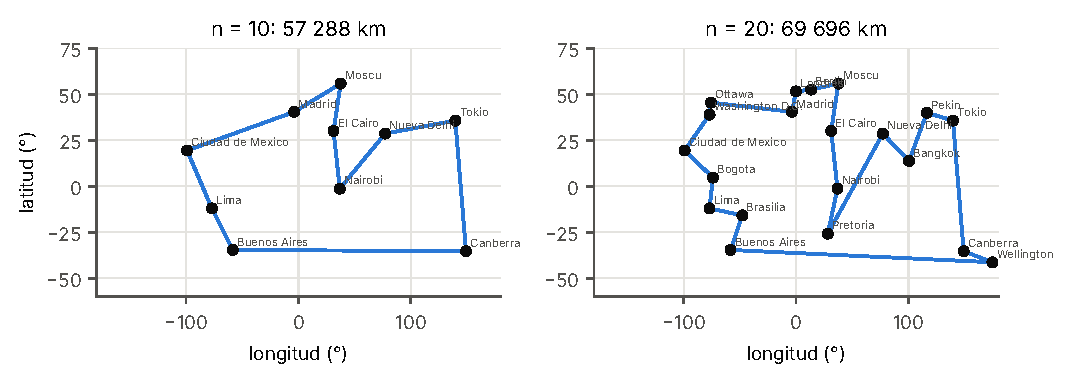
\includegraphics[width=\textwidth]{../figuras/f11_rutas.pdf}
\caption{Rutas óptimas para $n=10$ y $n=20$ (proyección equirectangular). Ambas parten y terminan en Lima.}
\label{fig:rutas}
\end{figure}

\subsection{Tiempo secuencial frente a la complejidad teórica}

La Tabla~\ref{tab:v1} y las Figuras~\ref{fig:tn} y~\ref{fig:nodos} resumen la versión secuencial. Hay tres resultados principales.

\begin{enumerate}
    \item \textbf{La poda es la que hace viable el problema.} El peor caso $e\,(n-1)!$ de la Sección~\ref{sec:compl_sec} predice $3.3\times10^{17}$ nodos para $n=20$, pero v1 explora $5.0\times10^{8}$: una fracción de $1.5\times10^{-9}$. Esa fracción disminuye a medida que $n$ crece (de $4.4\times10^{-3}$ con $n=10$ a $1.5\times10^{-9}$ con $n=20$), porque la mejor solución encontrada descarta ramas cada vez más grandes.
    \item \textbf{El costo por nodo sigue el $O(n^2)$ del PRAM.} Dividiendo $T_1$ entre $N(n)$ se obtiene un costo por nodo que se ajusta a $c\,n^2$ con $c \approx 2.0$~ns, que es el costo de \textsc{CalcularBound}. Así, $T_1(n) \approx c\,n^2\,N(n)$, que es la misma expresión del trabajo $W(n)$ de la Tabla~\ref{tab:costos} con $N(n)$ medido en lugar del peor caso.
    \item \textbf{Ajuste de una función a los tiempos.} Ajustando por mínimos cuadrados sobre $\log T_1$ se obtiene el polinomio
    \[
    T_1(n) \approx 1.09\times10^{-22}\; n^{18.5} \ \text{s}, \qquad R^2 = 0.978,
    \]
    y la exponencial $T_1(n) \approx 1.74\times10^{-9}\cdot 3.62^{\,n}$~s, con $R^2 = 0.996$. Ninguna se parece a $n!$: de $n=19$ a $n=20$, $n!$ crece $20\times$, mientras que el tiempo medido crece $7.2\times$. Sin embargo, el exponente $k = 18.5$ indica que, en el rango medido, el comportamiento sigue siendo exponencial: la poda reduce enormemente la base del crecimiento, pero no lo vuelve polinomial. Esto es consistente con que el TSP sea NP-difícil.
\end{enumerate}

\begin{figure}[H]
\centering
\begin{minipage}{0.49\textwidth}
\centering
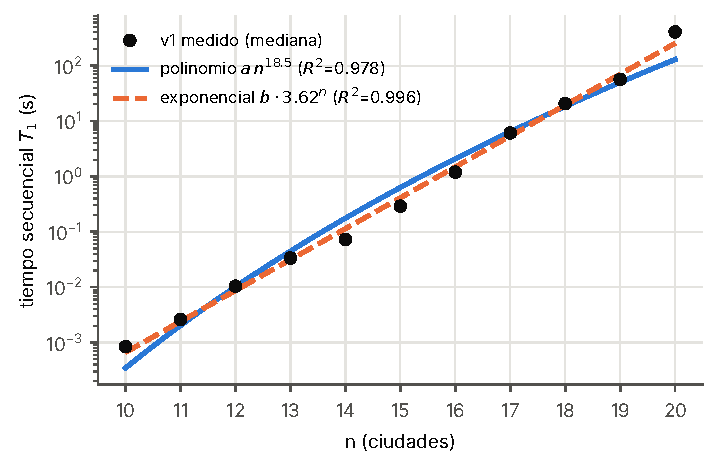
\includegraphics[width=\textwidth]{../figuras/f1_tiempo_vs_n.pdf}
\caption{$T_1(n)$ medido y funciones ajustadas.}
\label{fig:tn}
\end{minipage}\hfill
\begin{minipage}{0.49\textwidth}
\centering
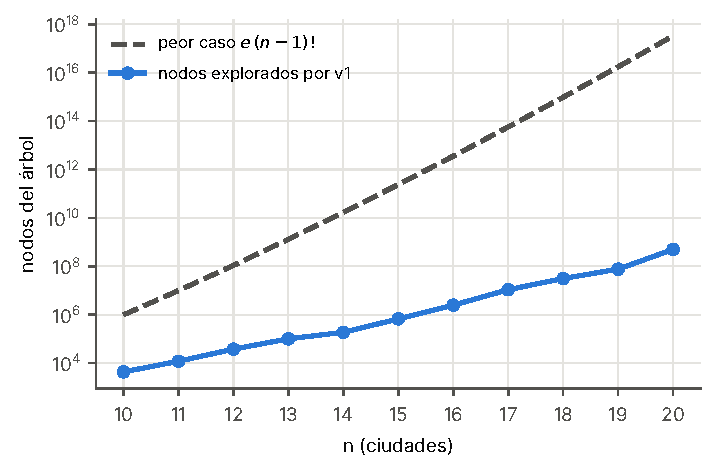
\includegraphics[width=\textwidth]{../figuras/f2_nodos_vs_n.pdf}
\caption{Nodos explorados por v1 frente al peor caso.}
\label{fig:nodos}
\end{minipage}
\end{figure}

\begin{table}[H]
\centering
\caption{Versión secuencial v1 (mediana de 5 ejecuciones; 3 para $n \ge 19$) en Khipu (nodo n003).}
\label{tab:v1}
\small
\begin{tabular}{rrrrrr}
\toprule
$n$ & $T_1$ & Nodos $N(n)$ & $N(n)/e(n-1)!$ & Costo óptimo (km) & GFLOP/s \\
\midrule
10 & 0.84~ms & 4\,316 & $4.4\times10^{-3}$ & 57\,288 & 0.62 \\
11 & 2.61~ms & 11\,900 & $1.2\times10^{-3}$ & 57\,346 & 0.68 \\
12 & 10.38~ms & 37\,509 & $3.5\times10^{-4}$ & 57\,680 & 0.74 \\
13 & 33.53~ms & 100\,553 & $7.7\times10^{-5}$ & 60\,054 & 0.85 \\
14 & 72.66~ms & 186\,497 & $1.1\times10^{-5}$ & 60\,862 & 1.06 \\
15 & 289.56~ms & 668\,905 & $2.8\times10^{-6}$ & 61\,186 & 1.18 \\
16 & 1.19~s & 2\,478\,672 & $7.0\times10^{-7}$ & 61\,225 & 1.25 \\
17 & 6.09~s & 10\,738\,854 & $1.9\times10^{-7}$ & 66\,655 & 1.28 \\
18 & 20.68~s & 31\,174\,281 & $3.2\times10^{-8}$ & 66\,690 & 1.34 \\
19 & 56.63~s & 75\,973\,548 & $4.4\times10^{-9}$ & 68\,751 & 1.37 \\
20 & 407.10~s & 496\,476\,459 & $1.5\times10^{-9}$ & 69\,696 & 1.39 \\
\bottomrule
\end{tabular}
\end{table}


\subsection{Speedup y eficiencia}

Las Figuras~\ref{fig:speedup} y~\ref{fig:eficiencia} muestran el speedup $S_p = T_{v1}/T_p$ y la eficiencia $E_p = S_p/p$ para $n = 16, 18, 20$. La Tabla~\ref{tab:n20} detalla el caso $n=20$. El mejor resultado es un speedup de 9.0 con v3 y $p=16$ (45~s frente a 407~s), es decir, una eficiencia de 0.57.

\begin{figure}[H]
\centering
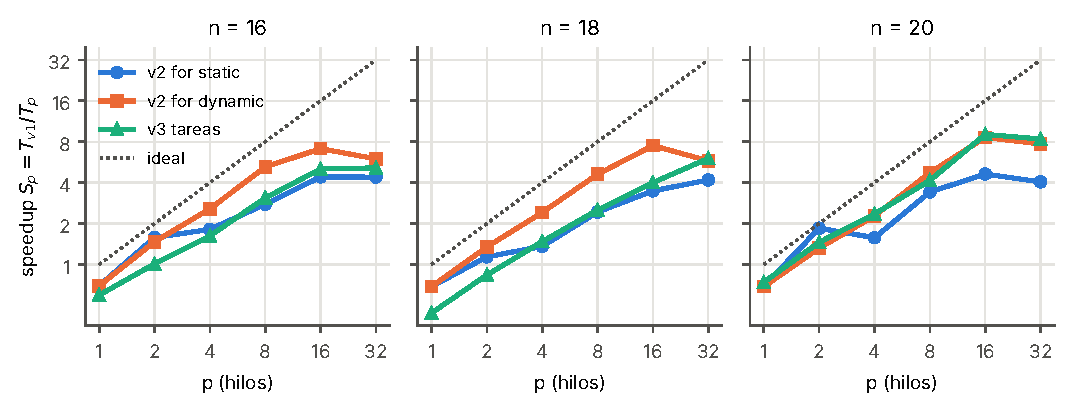
\includegraphics[width=\textwidth]{../figuras/f3_speedup.pdf}
\caption{Speedup respecto de v1 (escala $\log_2$). La línea punteada es el speedup ideal $S_p = p$.}
\label{fig:speedup}
\end{figure}

\begin{figure}[H]
\centering
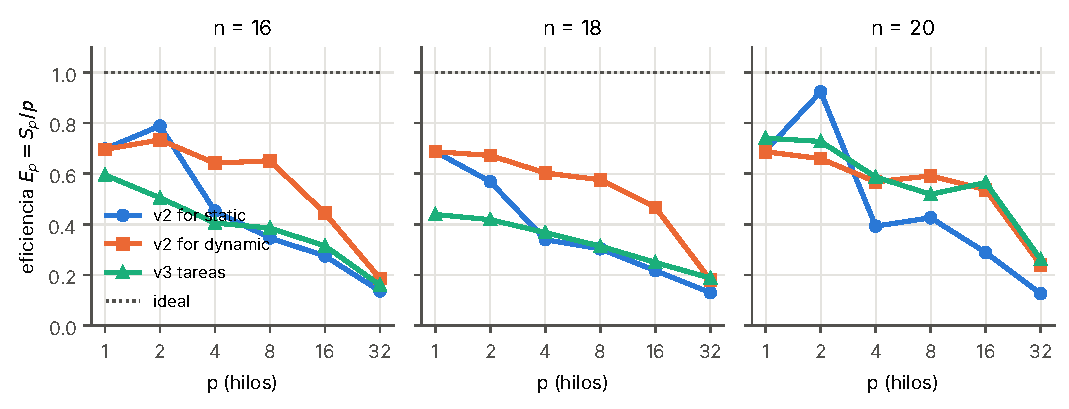
\includegraphics[width=\textwidth]{../figuras/f4_eficiencia.pdf}
\caption{Eficiencia $E_p = S_p/p$.}
\label{fig:eficiencia}
\end{figure}

\begin{table}[H]
\centering
\caption{Resultados para $n=20$ ($T_{v1} = 407.1$~s). $S_p = T_{v1}/T_p$, $E_p = S_p/p$, $S^{rel}_p = T^{(v)}_1/T^{(v)}_p$ y $\sigma_p$ = nodos adicionales respecto de v1.}
\label{tab:n20}
\small
\begin{tabular}{llrrrrr}
\toprule
Versión & $p$ & $T_p$ (s) & $S_p$ & $E_p$ & $S^{rel}_p$ & $\sigma_p$ \\
\midrule
v2 static & 1 & 588.9 & 0.69 & 0.69 & 1.00 & 0.000 \\
 & 2 & 220.4 & 1.85 & 0.92 & 2.67 & -0.380 \\
 & 4 & 258.9 & 1.57 & 0.39 & 2.27 & +0.030 \\
 & 8 & 119.4 & 3.41 & 0.43 & 4.93 & -0.226 \\
 & 16 & 88.0 & 4.63 & 0.29 & 6.69 & +0.131 \\
 & 32 & 100.6 & 4.05 & 0.13 & 5.85 & +0.273 \\
\midrule
v2 dynamic & 1 & 592.7 & 0.69 & 0.69 & 1.00 & 0.000 \\
 & 2 & 308.5 & 1.32 & 0.66 & 1.92 & +0.001 \\
 & 4 & 179.1 & 2.27 & 0.57 & 3.31 & +0.099 \\
 & 8 & 86.0 & 4.74 & 0.59 & 6.89 & +0.182 \\
 & 16 & 47.4 & 8.59 & 0.54 & 12.50 & +0.059 \\
 & 32 & 52.9 & 7.70 & 0.24 & 11.21 & +0.120 \\
\midrule
v3 tareas & 1 & 549.7 & 0.74 & 0.74 & 1.00 & +0.009 \\
 & 2 & 279.7 & 1.46 & 0.73 & 1.97 & -0.040 \\
 & 4 & 173.3 & 2.35 & 0.59 & 3.17 & +0.019 \\
 & 8 & 98.1 & 4.15 & 0.52 & 5.61 & +0.219 \\
 & 16 & 45.0 & 9.05 & 0.57 & 12.22 & -0.051 \\
 & 32 & 48.6 & 8.38 & 0.26 & 11.31 & +0.070 \\
\bottomrule
\end{tabular}
\end{table}


La diferencia con el speedup ideal se debe a cuatro efectos, que se pueden separar con los contadores del código:

\begin{enumerate}
    \item \textbf{Costo del código OpenMP con un solo hilo.} Con $p=1$, v2 explora exactamente los mismos nodos y hace los mismos FLOPs que v1, pero en Khipu tarda $1.44\times$ más (589~s frente a 407~s con $n=20$); la diferencia es igual en todas las repeticiones y en todos los $n$. Por eso $E_1 \approx 0.69$ y todas las eficiencias quedan por debajo de ese valor. Si se toma como referencia la propia versión con $p=1$ (speedup relativo, Figura~\ref{fig:relativo}), v2 dinámico y v3 alcanzan $12.5$ y $12.2$ con $p=16$, lo que equivale a eficiencias de 0.78 y 0.76. La Sección~\ref{sec:diag} muestra que este sobrecosto no es propio de OpenMP sino de la afinidad: el mismo binario tarda lo mismo que v1 cuando el hilo no se fija a un núcleo.
    \item \textbf{Desbalance de carga en el reparto estático.} La poda hace que unos prefijos se descarten casi de inmediato y otros contengan la mayor parte del trabajo. Con \texttt{schedule(static)} cada hilo recibe un bloque fijo de prefijos y debe esperar al más cargado: v2 estático no pasa de un speedup de 4.6. Con reparto dinámico o con tareas, los hilos que terminan toman más trabajo, y el speedup sube a 8.6--9.0.
    \item \textbf{Search overhead ($\sigma_p$).} Como los hilos no ven a la vez la mejor solución que encuentran los demás, la versión paralela suele explorar más nodos que v1: hasta un 22\% más con v3 y $p=8$ (Tabla~\ref{tab:n20}). También aparece el efecto contrario: v2 estático con $p=2$ explora un 38\% \emph{menos} nodos, porque uno de los hilos encuentra temprano una ruta buena que poda las ramas del otro. Por eso su speedup relativo es superlineal (2.67 con 2 hilos). Estas son las anomalías de Branch and Bound paralelo mencionadas en la Sección~\ref{sec:paralelo}.
    \item \textbf{Pasar de 16 a 32 hilos casi no ayuda.} Con v2 dinámico el speedup baja entre un 9\% y un 27\% para todo $n \ge 14$; v2 estático y v3 mejoran en algunos $n$ (hasta $1.5\times$ con v3 y $n=18$) y empeoran en otros. El modelo de overhead no explica esta caída (Sección~\ref{sec:res_modelo}). La causa es el hardware asignado: con $p=32$ los hilos se reparten en los mismos 16 núcleos físicos que con $p=16$, dos por núcleo (Sección~\ref{sec:diag}).
\end{enumerate}

\begin{figure}[H]
\centering
\begin{minipage}{0.49\textwidth}
\centering
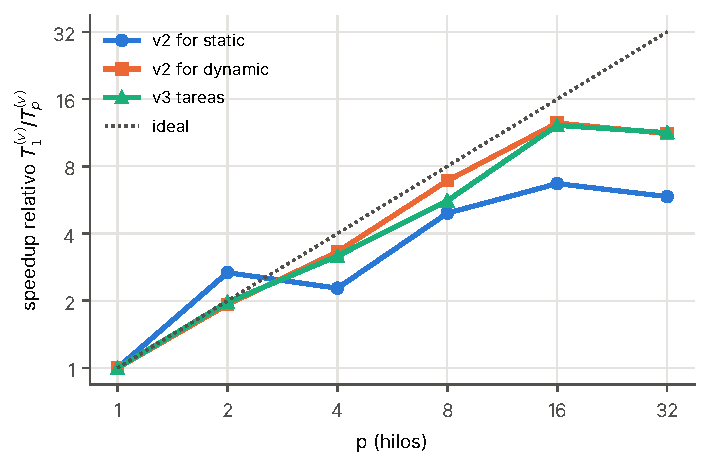
\includegraphics[width=\textwidth]{../figuras/f5_speedup_relativo.pdf}
\caption{Speedup relativo a la propia versión con $p=1$ ($n=20$).}
\label{fig:relativo}
\end{minipage}\hfill
\begin{minipage}{0.49\textwidth}
\centering
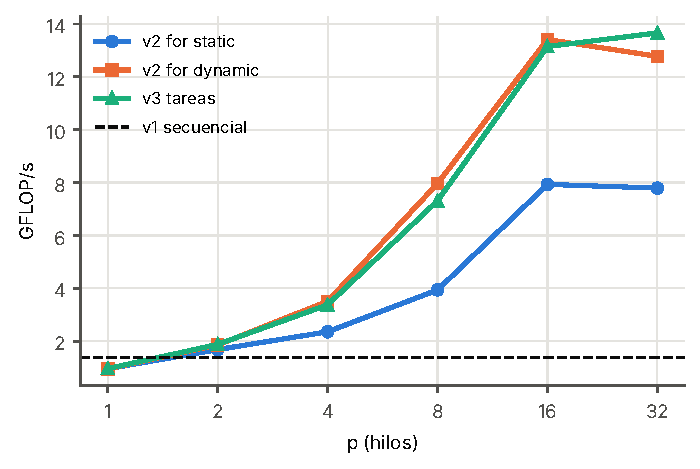
\includegraphics[width=\textwidth]{../figuras/f7_flops.pdf}
\caption{GFLOP/s frente a $p$ ($n=20$).}
\label{fig:flops}
\end{minipage}
\end{figure}

\subsection{FLOPs frente a $p$}
La Figura~\ref{fig:flops} muestra la tasa de FLOPs medida con el contador del código. v1 alcanza 1.39~GFLOP/s; las versiones paralelas suben de forma casi lineal hasta 13.4~GFLOP/s (v2 dinámico) y 13.0~GFLOP/s (v3) con $p=16$, y se estancan con 32 hilos, que comparten esos mismos 16 núcleos físicos. Como el número de FLOPs por ejecución varía poco con $p$ (cambia solo con $\sigma_p$), esta gráfica tiene la misma forma que la del speedup. La tasa por núcleo es baja porque el código es principalmente de control: la mayoría de los FLOPs contados son comparaciones seguidas de saltos condicionales, no operaciones aritméticas encadenadas.

\subsection{Modelo de tiempo con overhead}
\label{sec:res_modelo}

La Figura~\ref{fig:overhead} muestra las componentes del overhead medidas con los \textit{microbenchmarks}: todas son del orden de microsegundos y crecen con $p$ (por ejemplo, $t_{tarea}$ pasa de 0.014~µs con 1 hilo a 15~µs con 32). Con $n = 20$, v3 crea 357 tareas y hace alrededor de 110 actualizaciones de la mejor solución, por lo que
\[
T_0(20, 32) = t_{fork} + N_{tar}\,t_{tarea} + U\,t_{crit} + d\,t_{bar} \approx 5~\text{ms},
\]
que es alrededor del 0.01\% de los 48.6~s que tarda esa ejecución. La Figura~\ref{fig:modelo} compara el tiempo medido con el modelo $T_p = T^{(v)}_1 (1+\sigma_p)/\big(p\,(1+\sigma_1)\big) + T_0$, usando $\sigma_p$ medido. Para v2 dinámico el modelo acierta hasta $p = 8$ (86.0~s medido frente a 87.6~s predicho), pero predice 21~s con $p=32$ frente a 53~s medidos. La conclusión es que, para este problema, los costos de crear hilos y tareas y de la sección crítica son despreciables: lo que limita la eficiencia es el desbalance de carga (v2 estático queda lejos del modelo desde $p=4$) y, con 32 hilos, que el job solo dispone de 16 núcleos físicos (Sección~\ref{sec:diag}).

\begin{figure}[H]
\centering
\begin{minipage}{0.49\textwidth}
\centering
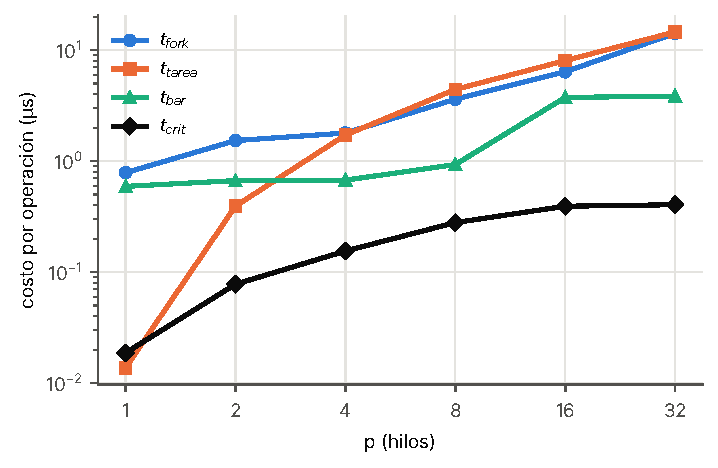
\includegraphics[width=\textwidth]{../figuras/f9_overhead.pdf}
\caption{Componentes del overhead de OpenMP en n003.}
\label{fig:overhead}
\end{minipage}\hfill
\begin{minipage}{0.49\textwidth}
\centering
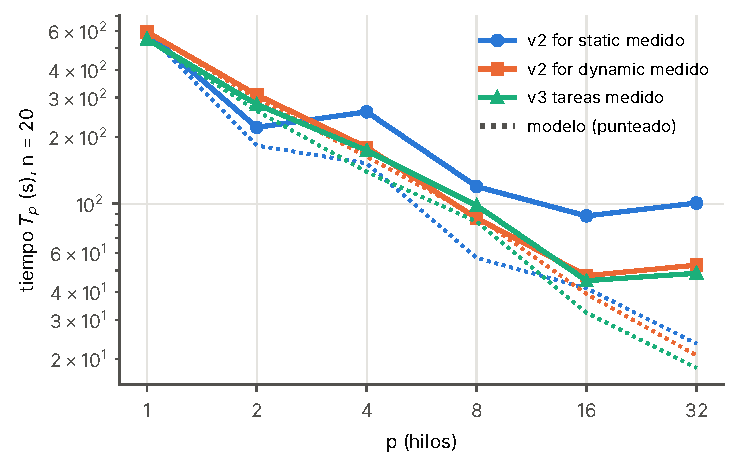
\includegraphics[width=\textwidth]{../figuras/f10_modelo_vs_medido.pdf}
\caption{$T_p$ medido (línea continua) y modelo (punteada), $n=20$.}
\label{fig:modelo}
\end{minipage}
\end{figure}

\subsection{Diagnóstico de la asignación de núcleos}
\label{sec:diag}

Para explicar los dos efectos que el modelo no cubre (el sobrecosto con $p=1$ y la falta de mejora de 16 a 32 hilos), se ejecutó un job de diagnóstico (\texttt{slurm/diagnostico.slurm}) con la misma configuración que los experimentos, en el mismo nodo n003 y con las capitales, $n=18$. El job recibió las CPUs lógicas 12--27 y 44--59: 32 CPUs que corresponden a \textbf{16 núcleos físicos con dos hilos cada uno} (4 núcleos en el primer procesador y 12 en el segundo). La Tabla~\ref{tab:diag} muestra los tiempos.

\begin{table}[H]
\centering
\caption{Diagnóstico en n003, capitales con $n=18$ (una ejecución por fila). \texttt{cores}/\texttt{threads}: un hilo de OpenMP por núcleo físico o por CPU lógica; \texttt{close}/\texttt{spread}: hilos juntos o repartidos.}
\label{tab:diag}
\small
\begin{tabular}{lll r}
\toprule
Prueba & Binario & Afinidad & $T$ (s) \\
\midrule
$p=1$ & v1 sin OpenMP & (sin fijar) & 23.1 \\
 & v1 compilado con OpenMP & \texttt{cores}, \texttt{close} & 31.0 \\
 & v2 dinámico & \texttt{cores}, \texttt{close} & 31.4 \\
 & v2 dinámico & sin afinidad & 21.9 \\
\midrule
$p=16$, $d=3$ & v2 dinámico & \texttt{cores}, \texttt{close} & 1.83 \\
 & v2 dinámico & \texttt{cores}, \texttt{spread} & 1.86 \\
 & v2 dinámico & \texttt{threads}, \texttt{close} & 3.05 \\
 & v2 dinámico & sin afinidad & 4.79 \\
\midrule
$p=32$, $d=3$ & v2 dinámico & \texttt{cores}, \texttt{close} & 1.99 \\
 & v2 dinámico & \texttt{threads}, \texttt{close} & 1.91 \\
 & v2 dinámico & sin afinidad & 1.95 \\
\bottomrule
\end{tabular}
\end{table}

\begin{itemize}
    \item \textbf{De 16 a 32 hilos no hay más núcleos.} Con $p=16$ y un hilo por núcleo físico, v2 dinámico tarda 1.83~s. Con $p=32$ los hilos ocupan los mismos 16 núcleos de a dos, y el tiempo es prácticamente el mismo (1.9--2.0~s), con cualquier afinidad. En cambio, 16 hilos en solo 8 núcleos (dos por núcleo, \texttt{threads}) tardan 3.05~s: un par de hilos en el mismo núcleo rinde apenas un 20\% más que uno solo. Por eso, en todos los experimentos, $p=32$ no debe leerse como 32 núcleos sino como 16 núcleos con hyperthreading.
    \item \textbf{El sobrecosto con $p=1$ es de afinidad.} El mismo binario de v2 con $p=1$ tarda 31.4~s si el hilo se fija a un núcleo y 21.9~s si no, y la versión secuencial compilada con OpenMP (que también fija su hilo) tarda 31.0~s frente a 23.1~s sin OpenMP. Es la misma razón de $1.44\times$ observada en la primera tanda. Con \texttt{close}, el único hilo queda fijado al primer núcleo asignado, que está en el procesador donde el job solo tiene 4 de sus 16 núcleos. Una explicación consistente es que ese procesador estaba más cargado por otros trabajos del nodo, mientras que un hilo libre puede migrar al otro. Como las CPUs asignadas cambian de un job a otro, el efecto no apareció en la tanda VLSI.
    \item \textbf{Fijar los hilos sí importa con muchos hilos.} Sin afinidad, 16 hilos tardan 4.79~s, $2.6\times$ más que fijados a núcleos distintos, porque el sistema operativo puede ponerlos en el mismo núcleo físico.
    \item Con la profundidad $d=3$, v2 dinámico logra con 16 núcleos un speedup de $23.1/1.83 = 12.6$ ($E_{16}=0.79$) para $n=18$, frente a 7.5 con $d=2$ en la tanda principal (Figura~\ref{fig:speedup}).
\end{itemize}

\subsection{Escalabilidad con el tamaño del problema}

La Figura~\ref{fig:escal} muestra la eficiencia en función de $n$ con 8 y 16 hilos. Con $n=10$ la eficiencia no supera 0.15 en ninguna versión: v1 tarda menos de un milisegundo, del mismo orden que abrir la región paralela y crear las tareas. A medida que $n$ crece, el trabajo por hilo aumenta mucho más rápido que el overhead, y la eficiencia sube hasta estabilizarse alrededor de 0.6 con $p=8$ y entre 0.4 y 0.55 con $p=16$ (v2 dinámico). Es decir, el algoritmo escala mejor cuanto más grande es el problema, como predice la expresión de $E_p$ de la Sección~\ref{sec:paralelo}: el término $p\,(S + T_0)/W$ tiende a cero cuando $W$ crece.

\begin{figure}[H]
\centering
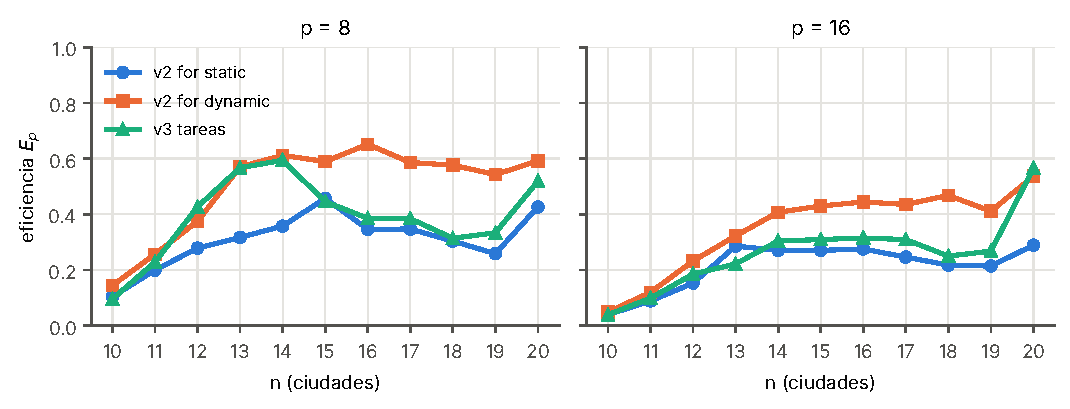
\includegraphics[width=\textwidth]{../figuras/f6_escalabilidad.pdf}
\caption{Eficiencia frente a $n$ con $p=8$ y $p=16$.}
\label{fig:escal}
\end{figure}

\subsection{Profundidad de corte}

Con $d=2$ y $n=16$ solo hay 210 prefijos para repartir entre 16 o 32 hilos, y los más pesados limitan el tiempo total. La Figura~\ref{fig:depth} muestra que aumentar a $d=3$ (2\,730 prefijos) reduce el tiempo de v2 dinámico con 16 hilos de 0.17~s a 0.105~s, lo que equivale a un speedup de 11.3 y una eficiencia de 0.71. Con $d=4$ deja de mejorar. En v3 el número de tareas crece de 15 ($d=1$) a 225, 2\,341 y 16\,884, y con $d=4$ y 16 hilos el tiempo vuelve a subir: crear tareas de grano demasiado fino ya no compensa. Para las corridas principales se usó $d=2$; con $d=3$ los speedups de la Tabla~\ref{tab:n20} probablemente serían mayores.

\begin{figure}[H]
\centering
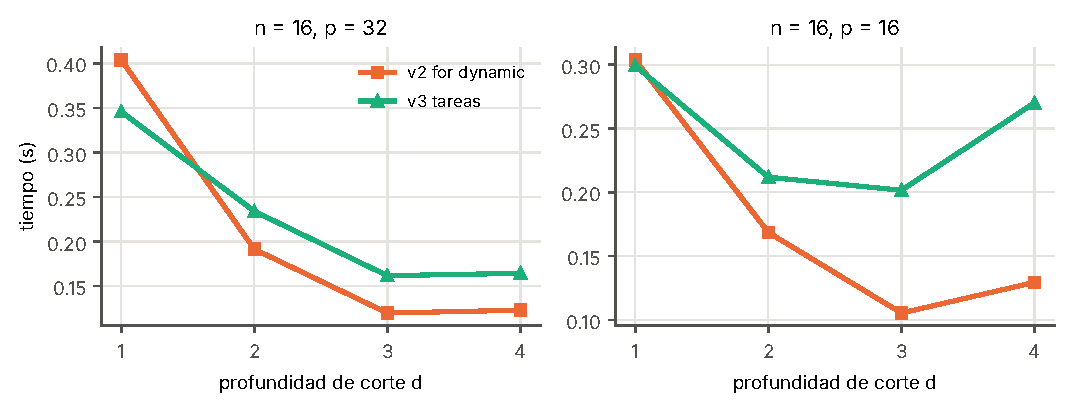
\includegraphics[width=\textwidth]{../figuras/f8_profundidad.pdf}
\caption{Efecto de la profundidad de corte $d$ para $n=16$.}
\label{fig:depth}
\end{figure}

\subsection{Instancias VLSI recortadas}
\label{sec:vlsi}

Como extensión se aplicó el mismo código a la otra opción del enunciado, la instancia VLSI \texttt{xqf131} \citep{cook_vlsi}, recortada como permite el enunciado. Los 131 puntos se ordenaron aleatoriamente con una semilla fija (2026), y la instancia de tamaño $n$ son los primeros $n$ puntos. Las distancias son euclidianas redondeadas al entero más cercano, como define TSPLIB. Como el óptimo publicado (564) corresponde a la instancia completa, cada instancia recortada se validó contra un algoritmo exacto independiente: la programación dinámica de Held--Karp \citep{held1962dynamic}, $O(n^2 2^n)$, implementada en \texttt{tsp\_dp.cpp}. Para $n=12,\dots,22$ en VLSI y $n=12,\dots,20$ en capitales, todas las versiones y ambas cotas coincidieron con Held--Karp. Esto extiende la validación de la Sección~\ref{sec:impl}, que con fuerza bruta solo llegaba a $n=11$.

La Tabla~\ref{tab:vlsi} y la Figura~\ref{fig:vlsi_t} resumen los resultados. Con la cota del Algoritmo~\ref{alg:bound}, las instancias VLSI son más difíciles que las capitales: con $n=20$, v1 explora $1.08\times10^{9}$ nodos y tarda 675~s, frente a $5.0\times10^{8}$ nodos y 407~s con las capitales. Una explicación probable es que los puntos VLSI están sobre una grilla y muchas distancias son iguales, lo que hace que la poda descarte menos ramas. En cambio, el paralelismo rinde mejor: v3 llega a un speedup de 12.4 con 32 hilos y v2 dinámico a 9.6 con 16 ($E_{16} = 0.60$). Este es el mejor resultado de todo el proyecto con la cota original (Figura~\ref{fig:vlsi_s}, izquierda).

En esta tanda, con la cota original y $p=1$, v2 es incluso entre un 3\% y un 6\% más rápida que v1 (para $n \ge 14$), en lugar de $1.44\times$ más lenta como con las capitales. Según el diagnóstico de la Sección~\ref{sec:diag}, esto depende de en qué núcleo queda fijado el único hilo, que cambia según las CPUs que SLURM asigna a cada job. Con v4, v2 con $p=1$ sí es entre un 6\% y un 12\% más lenta que v1 (para $n \ge 28$), por el costo de generar y recorrer los prefijos con $d=3$.

\begin{figure}[H]
\centering
\begin{minipage}{0.49\textwidth}
\centering
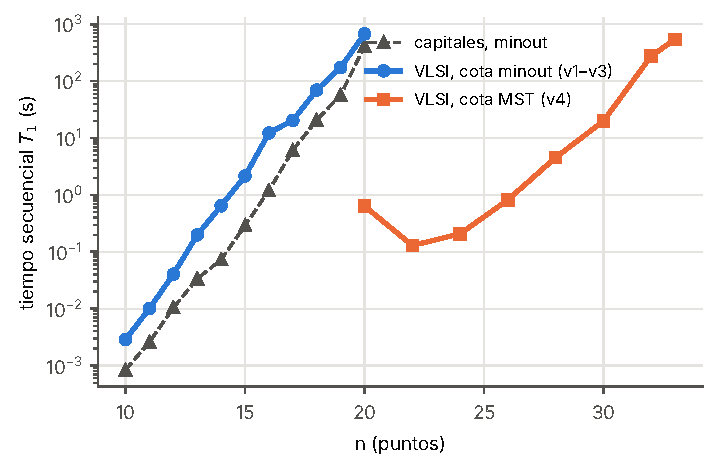
\includegraphics[width=\textwidth]{../figuras/f12_vlsi_tiempo.pdf}
\caption{$T_1(n)$ con ambas cotas (VLSI) y con la cota original (capitales).}
\label{fig:vlsi_t}
\end{minipage}\hfill
\begin{minipage}{0.49\textwidth}
\centering
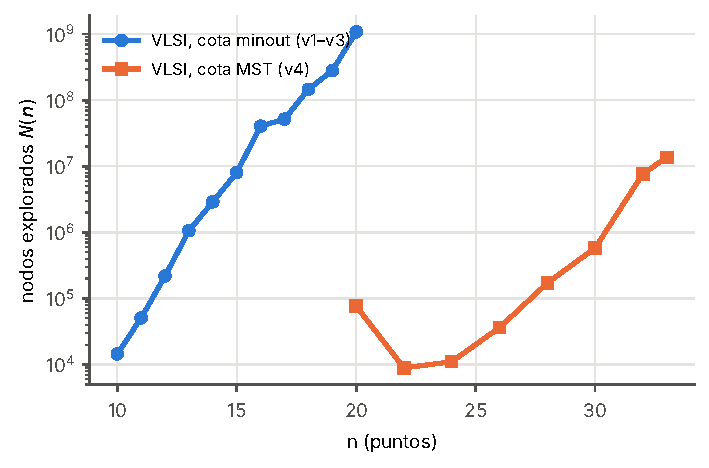
\includegraphics[width=\textwidth]{../figuras/f13_vlsi_nodos.pdf}
\caption{Nodos explorados por v1 con cada cota (VLSI).}
\label{fig:vlsi_n}
\end{minipage}
\end{figure}

\begin{table}[H]
\centering
\caption{Instancias VLSI recortadas (\texttt{xqf131}, primeras $n$ filas del orden aleatorio). $T_1$ y $N$ de v1 con la cota indicada; mejor speedup $S_p = T_{v1}/T_p$ entre las versiones paralelas.}
\label{tab:vlsi}
\small
\begin{tabular}{llrrrl}
\toprule
Cota & $n$ & $T_1$ & Nodos $N(n)$ & Costo óptimo & Mejor $S_p$ (versión, $p$) \\
\midrule
minout & 10 & 2.88~ms & 14\,471 & 209 & 3.8 (v2 dyn., 8) \\
 & 11 & 10.09~ms & 50\,610 & 218 & 5.9 (v2 dyn., 16) \\
 & 12 & 40.33~ms & 218\,309 & 218 & 7.8 (v2 dyn., 16) \\
 & 13 & 198.08~ms & 1\,059\,832 & 220 & 9.4 (v2 dyn., 16) \\
 & 14 & 641.96~ms & 2\,899\,284 & 221 & 9.3 (v2 dyn., 16) \\
 & 15 & 2.14~s & 8\,068\,716 & 223 & 10.7 (v2 dyn., 16) \\
 & 16 & 12.24~s & 40\,495\,673 & 224 & 11.8 (v3, 32) \\
 & 17 & 20.33~s & 51\,890\,797 & 236 & 11.6 (v3, 32) \\
 & 18 & 69.74~s & 146\,186\,647 & 253 & 11.9 (v3, 32) \\
 & 19 & 172.32~s & 280\,775\,761 & 254 & 11.6 (v3, 16) \\
 & 20 & 674.65~s & 1\,081\,131\,042 & 257 & 12.4 (v3, 32) \\
\midrule
MST (v4) & 20 & 635.38~ms & 76\,415 & 257 & 11.9 (v3, 32) \\
 & 22 & 129.07~ms & 8\,893 & 271 & 5.5 (v3, 32) \\
 & 24 & 206.36~ms & 11\,040 & 278 & 4.5 (v3, 16) \\
 & 26 & 818.48~ms & 36\,275 & 281 & 4.9 (v3, 32) \\
 & 28 & 4.53~s & 171\,088 & 285 & 7.7 (v2 dyn., 32) \\
 & 30 & 19.83~s & 580\,308 & 294 & 8.8 (v2 dyn., 16) \\
 & 32 & 276.21~s & 7\,700\,054 & 304 & 7.7 (v2 dyn., 16) \\
 & 33 & 542.39~s & 13\,642\,732 & 305 & 7.8 (v2 dyn., 16) \\
\bottomrule
\end{tabular}
\end{table}


\subsection{v4: cota por árbol de expansión mínima}

Con la cota MST, la instancia VLSI con $n=20$ se resuelve con 76\,415 nodos en 0.64~s, frente a $1.08\times10^{9}$ nodos y 675~s con la cota original: $14\,000$ veces menos nodos y $1\,060$ veces menos tiempo. Cada nodo cuesta unas 13 veces más (Prim recorre las ciudades pendientes dos veces por iteración), pero la poda compensa con creces. Esto permite resolver de forma exacta instancias de hasta $n=33$ en 9~minutos de forma secuencial y en 70~s con 16 hilos (Figura~\ref{fig:vlsi_r}). Para $n=33$, Held--Karp necesitaría unos $2^{32}\cdot 32$ estados (más de 1~TB de memoria), así que en ese rango el Branch and Bound con buena cota es el único método exacto viable de los dos. El número de nodos no crece de forma monótona: la instancia $n=20$ resulta más difícil que la $n=22$, porque depende de dónde caen los puntos y no solo de cuántos son.

\begin{figure}[H]
\centering
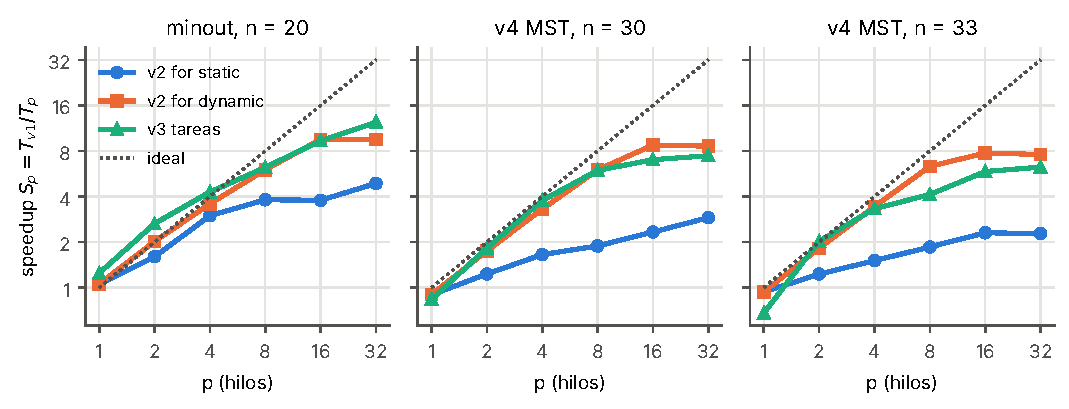
\includegraphics[width=\textwidth]{../figuras/f14_vlsi_speedup.pdf}
\caption{Speedup en VLSI: cota original con $n=20$ y v4 con $n=30$ y $n=33$.}
\label{fig:vlsi_s}
\end{figure}

En paralelo (Figuras~\ref{fig:vlsi_s} y~\ref{fig:vlsi_e}), v4 confirma las conclusiones anteriores con más fuerza:

\begin{itemize}
    \item \textbf{El reparto estático no funciona con una poda fuerte.} Con la cota MST la mayoría de los prefijos se descarta casi de inmediato, y v2 estático no supera un speedup de 2.3 para $n=33$, mientras que v2 dinámico llega a 7.8 con 16 hilos ($E_{16}=0.48$) y a 8.8 para $n=30$.
    \item \textbf{El orden de exploración importa.} v3 con $p=1$ explora un 49\% más nodos que v1 para $n=33$: al crear como tareas todos los hijos de los primeros niveles antes de explorarlos, la búsqueda tarda más en encontrar rutas buenas que poden el resto. v2 dinámico, que recorre los prefijos en el mismo orden que v1, no tiene ese problema y es la mejor opción para v4 con $n \ge 28$.
    \item \textbf{La eficiencia depende de que haya trabajo suficiente.} Entre $n=22$ y $n=26$, v4 termina en menos de un segundo y la eficiencia con 16 hilos baja a 0.2--0.3. Desde $n=28$, cuando el tiempo secuencial supera algunos segundos, se mantiene cerca de 0.5 con v2 dinámico.
    \item Con 32 hilos el tiempo de v2 dinámico vuelve a estancarse, igual que con las capitales y por la misma razón: dos hilos por núcleo físico.
\end{itemize}

\begin{figure}[H]
\centering
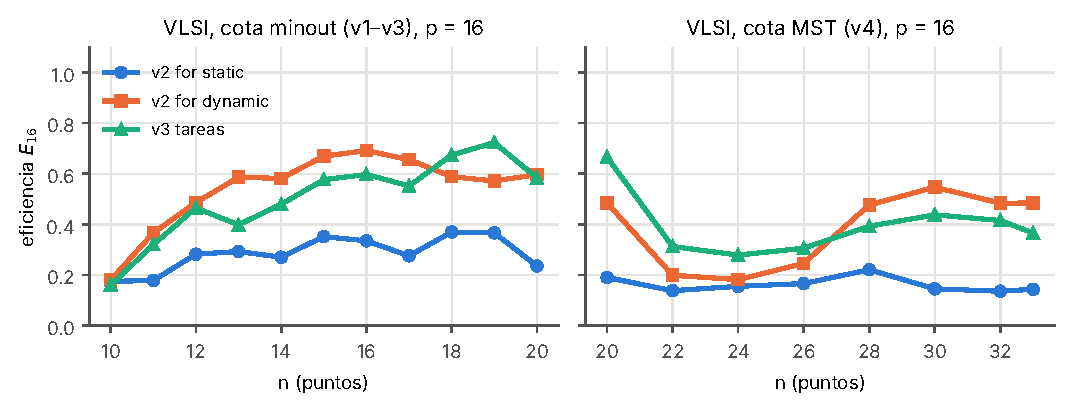
\includegraphics[width=\textwidth]{../figuras/f15_vlsi_eficiencia.pdf}
\caption{Eficiencia con 16 hilos en función de $n$ (VLSI).}
\label{fig:vlsi_e}
\end{figure}

\begin{figure}[H]
\centering
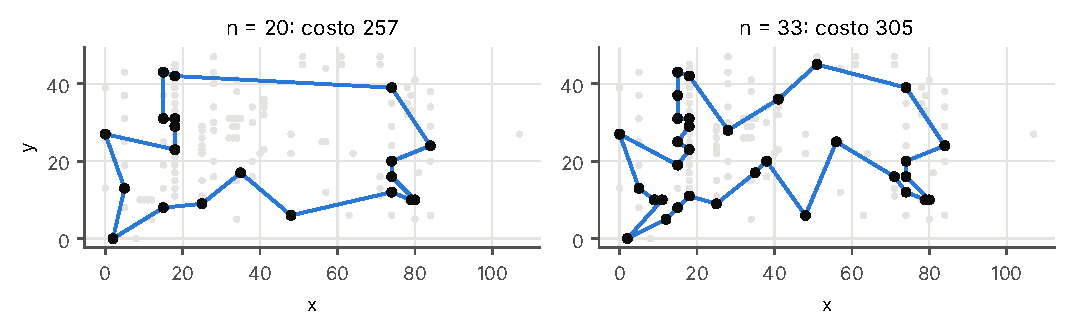
\includegraphics[width=\textwidth]{../figuras/f16_vlsi_rutas.pdf}
\caption{Rutas óptimas VLSI para $n=20$ y $n=33$. En gris, los 131 puntos de \texttt{xqf131}.}
\label{fig:vlsi_r}
\end{figure}

\subsection{Resumen de escalabilidad: $T_s/T_p$ frente a $n$ y regresión}
\label{sec:escal_reg}

La Figura~\ref{fig:speedup_n} reúne los tres casos estudiados en una sola vista: el speedup $T_s/T_p$ de v2 dinámico en función del tamaño $n$, con una curva por cada $p$. En los tres, para $p$ fijo el speedup crece con $n$ hasta estabilizarse. Con las capitales y 16 núcleos pasa de 0.8 con $n=10$ a 6.5 con $n=14$ y a 8.6 con $n=20$. Con VLSI y la cota original llega a 11 en $n=16$ y se mantiene entre 9 y 10.5. Con v4, el speedup baja entre $n=22$ y $n=26$, donde cada ejecución dura menos de un segundo, y sube a 7.7--8.8 desde $n=28$. Con $p=32$ (línea discontinua) los valores son prácticamente los de $p=16$, por el hyperthreading (Sección~\ref{sec:diag}). En las capitales, los valores con $p = 2$ y $4$ quedan por debajo de lo esperado por el sobrecosto de afinidad de esa tanda: el speedup relativo a la propia v2 con $p=1$ es 1.9 con $p=2$ para $n=20$.

\begin{figure}[H]
\centering
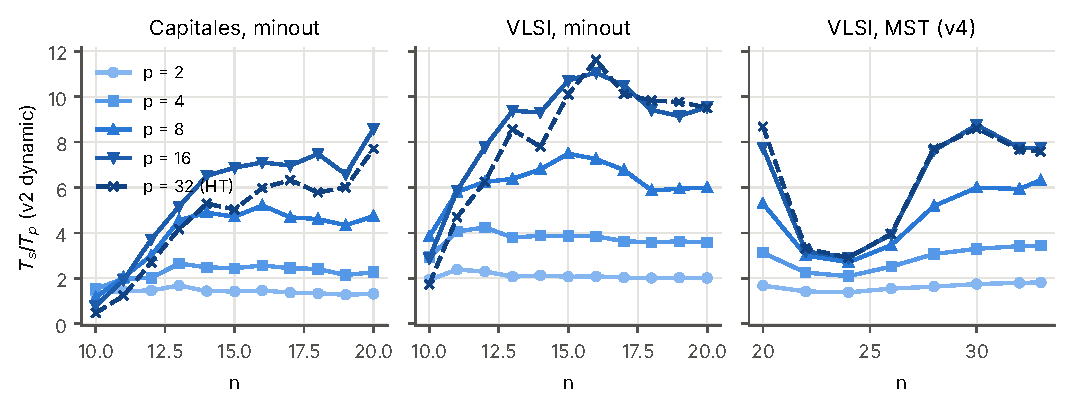
\includegraphics[width=\textwidth]{../figuras/f17_speedup_vs_n.pdf}
\caption{$T_s/T_p$ en función de $n$ para cada $p$ (v2 dinámico; $T_s$ es v1). Izquierda y centro: cota original ($d=2$); derecha: v4 ($d=3$).}
\label{fig:speedup_n}
\end{figure}

Para describir $T_s$ y $T_p$ con una sola expresión y cuantificar la escalabilidad, se ajustó por mínimos cuadrados sobre $\log T$ el modelo
\[
T_p(n) = \frac{a\,c^{\,n}}{p^{\beta}} + T_0 ,
\]
usando $T_s$ (v1) como el caso $p=1$ y v2 dinámico para $p = 2, 4, 8, 16$. No se incluye $p=32$, porque no agrega núcleos físicos. Cada parámetro tiene una interpretación directa:

\begin{itemize}
    \item $c$ es la base del crecimiento exponencial: cuánto se multiplica el tiempo al agregar una ciudad.
    \item $\beta$ mide la escalabilidad con el número de núcleos: $\beta = 1$ es el speedup ideal $p$, y cuando $T_0$ es despreciable la eficiencia tiende a $E_p = p^{\beta - 1}$.
    \item $T_0$ es la parte constante del término de overhead $T_0(n,p)$ de la Sección~\ref{sec:overhead}: el costo fijo que no se reduce al agregar núcleos.
\end{itemize}

La Tabla~\ref{tab:regresion} muestra los parámetros y la Figura~\ref{fig:regresion} compara el modelo con las mediciones. El ajuste es bueno en los tres casos ($R^2 \ge 0.99$ sobre $\log T$; el error típico es un factor de 1.3 sobre tiempos que abarcan cinco órdenes de magnitud).

\begin{table}[H]
\centering
\caption{Regresión de escalabilidad. Modelo conjunto $T_p(n) = a\,c^{\,n}/p^{\beta} + T_0$ ajustado por mínimos cuadrados sobre $\log T$ (v1 para $p=1$ y v2 dinámico para $p = 2, \dots, 16$). $E_{16}^{\infty} = 16^{\beta-1}$ es la eficiencia con 16 núcleos cuando $T_0$ es despreciable. A la derecha, la base de crecimiento $c_p$ de un ajuste exponencial $T_p(n) = a_p\,c_p^{\,n}$ separado para cada $p$.}
\label{tab:regresion}
\small
\setlength{\tabcolsep}{4pt}
\begin{tabular}{lcrrrrr|rrrrr}
\toprule
 & & \multicolumn{5}{c|}{Modelo conjunto} & \multicolumn{5}{c}{$c_p$ por separado} \\
Caso & $n$ & $c$ & $\beta$ & $T_0$ & $R^2$ & $E_{16}^{\infty}$ & $p{=}1$ & 2 & 4 & 8 & 16 \\
\midrule
Capitales, minout & 10--20 & 3.83 & 0.73 & 0.76~ms & 0.995 & 0.47 & 3.62 & 3.65 & 3.53 & 3.26 & 3.02 \\
VLSI, minout & 10--20 & 3.40 & 0.78 & 0.19~ms & 0.994 & 0.55 & 3.42 & 3.45 & 3.43 & 3.35 & 3.16 \\
VLSI, MST (v4) & 26--33 & 2.75 & 0.83 & 0.18~s & 0.990 & 0.62 & 2.59 & 2.52 & 2.48 & 2.40 & 2.39 \\
\bottomrule
\end{tabular}
\end{table}


\begin{figure}[H]
\centering
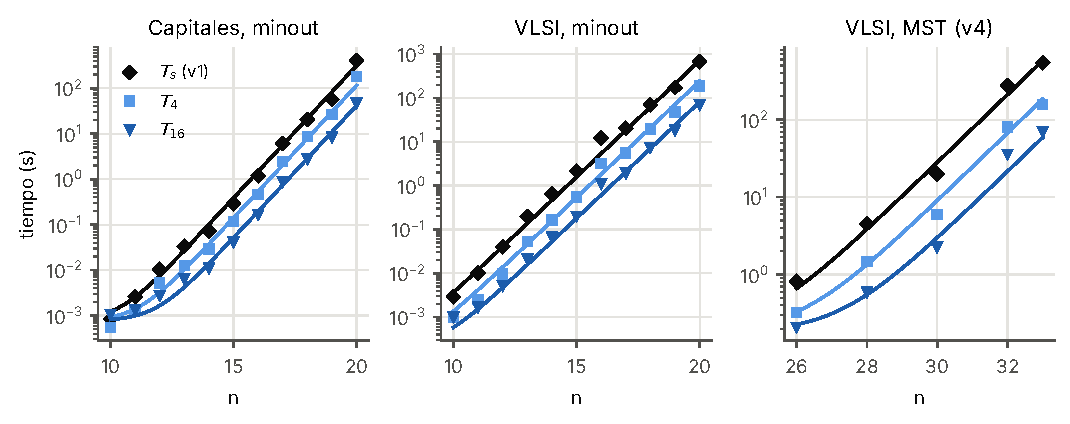
\includegraphics[width=\textwidth]{../figuras/f18_regresion.pdf}
\caption{Regresión de escalabilidad: tiempos medidos (puntos) y modelo $T_p(n) = a\,c^{\,n}/p^{\beta} + T_0$ (líneas) para $p = 1$ (v1), 4 y 16. En v4 el ajuste usa $n \ge 26$.}
\label{fig:regresion}
\end{figure}

De la regresión se concluye lo siguiente:
\begin{itemize}
    \item \textbf{Escalabilidad con los núcleos.} $\beta$ vale entre 0.73 y 0.83, es decir, $T_p$ disminuye como $p^{-0.73}$ a $p^{-0.83}$ y no como $p^{-1}$. Con 16 núcleos, la eficiencia asintótica que predice el modelo ($E_{16}^{\infty}$ = 0.47--0.62) es del mismo orden que la medida en los $n$ más grandes (0.48--0.60). La pérdida respecto del ideal no viene de $T_0$, sino del desbalance de carga y del search overhead (Secciones~\ref{sec:res_modelo} y~\ref{sec:vlsi}).
    \item \textbf{El término fijo $T_0$.} Con la cota original, $T_0$ es de 0.76~ms (capitales) y 0.19~ms (VLSI), del mismo orden que abrir la región paralela y repartir los prefijos (Figura~\ref{fig:overhead}). Por eso solo importa en las instancias pequeñas: con 16 núcleos, $T_0$ representa menos del 10\% del trabajo paralelo a partir de $n \approx 14$ en capitales y $n \approx 11$ en VLSI, que es justo donde el speedup de la Figura~\ref{fig:speedup_n} deja de subir rápido. En v4, $T_0 = 0.18$~s. Corresponde a la parte secuencial de v2 con $d=3$: los $32 \cdot 31 \cdot 30 = 29\,760$ prefijos de $n=33$, cada uno con una cota MST, se generan antes de la región paralela.
    \item \textbf{Escalabilidad con el tamaño del problema.} Si se ajusta $T_p(n) = a_p\,c_p^{\,n}$ por separado para cada $p$ (columnas de la derecha de la Tabla~\ref{tab:regresion}), la base $c_p$ disminuye con $p$: en las capitales, de 3.62 en secuencial a 3.02 con 16 núcleos. El tiempo paralelo crece más despacio que el secuencial, así que $T_s/T_p \propto (c_1/c_p)^n$ aumenta con $n$: los problemas más grandes aprovechan mejor los núcleos. Es lo que se espera de un algoritmo cuyo trabajo crece mucho más rápido que su overhead, y explica la forma de la Figura~\ref{fig:speedup_n}. Sin embargo, la eficiencia queda acotada por $p^{\beta-1}$, así que no se puede mantener constante al aumentar $p$ indefinidamente solo con agrandar el problema.
\end{itemize}

\subsection{Mejoras propuestas}
\begin{itemize}
    \item \textbf{Cota más ajustada (implementada en v4).} La cota MST redujo los nodos en cuatro órdenes de magnitud (Sección~\ref{sec:vlsi}). El siguiente paso sería la cota de Held--Karp por relajación lagrangiana (1-\textit{trees} con pesos en los nodos), que es todavía más ajustada. Con la cota original, arrancar con la solución de vecino más cercano casi no ayudó ($n=17$ capitales: sin cambio en los nodos), porque la limitación estaba en la cota.
    \item \textbf{Aprovechar la simetría.} Fijar el sentido del recorrido (por ejemplo, exigir que la segunda ciudad tenga un índice menor que la última) eliminaría la mitad de las rutas.
    \item \textbf{Reparto más fino y adaptativo.} Usar un corte que dependa de $n$ y de $p$, o un esquema de robo de trabajo, para reducir el desbalance. En v3, explorar primero el hijo más prometedor antes de crear el resto de las tareas evitaría el aumento de nodos observado con v4.
    \item \textbf{Asignación de núcleos.} Pedir núcleos físicos completos (con la opción \texttt{-{}-hint=}\allowbreak\texttt{nomultithread} de SLURM o un nodo exclusivo) para medir con 32 núcleos reales, y fijar los hilos con \texttt{OMP\_PROC\_BIND} solo cuando $p > 1$.
    \item \textbf{Versión distribuida con MPI.} Repartir los prefijos entre varios nodos de Khipu y difundir la mejor solución periódicamente permitiría usar más de 32 núcleos.
\end{itemize}

\section{Conclusiones}
\begin{itemize}
    \item Todas las versiones obtienen el óptimo exacto, validado contra fuerza bruta ($n \le 11$) y contra Held--Karp ($n \le 22$). La ruta mínima entre las 20 capitales mide 69\,696~km, frente a 57\,288~km con 10.
    \item El análisis PRAM se cumple en el costo por nodo ($\approx 2.0$~ns$\cdot n^2$), pero el número de nodos está muy por debajo del peor caso factorial: con $n=20$ se explora una fracción de $1.5\times10^{-9}$ del árbol. Aun así, el tiempo crece de forma exponencial ($3.62^n$, o un polinomio de grado 18.5 en el rango medido).
    \item El mejor speedup fue de 9.0 con 16 hilos (v3 con tareas, $n=20$), y de 11.3 con v2 dinámico y $d=3$ para $n=16$. El reparto dinámico o por tareas casi duplica el speedup del reparto estático, por el desbalance de carga que produce la poda.
    \item Los costos de crear hilos y tareas y de la sección crítica, medidos con \textit{microbenchmarks}, son de microsegundos y representan alrededor del 0.01\% del tiempo. Las pérdidas de eficiencia se deben al desbalance de carga, al search overhead ($\sigma_p$ entre $-0.38$ y $+0.27$) y a que con 32 hilos se comparten 16 núcleos físicos por hyperthreading. El sobrecosto de $1.44\times$ con un hilo se debió a la afinidad, no a OpenMP.
    \item La eficiencia aumenta con $n$: el algoritmo paralelo solo vale la pena a partir de $n \approx 13$, cuando el tiempo secuencial supera las decenas de milisegundos. La regresión $T_p(n) = a\,c^{\,n}/p^{\beta} + T_0$ describe todos los tiempos con $R^2 \ge 0.99$: $\beta = 0.73$--$0.83$ cuantifica la escalabilidad con los núcleos, y $T_p$ crece con una base menor que $T_s$ (3.02 frente a 3.62 por ciudad con 16 núcleos), por lo que el speedup crece con el tamaño del problema.
    \item En las instancias VLSI, el paralelismo rinde más (speedup de 12.4 con v3 y 32 hilos para $n=20$). La cota MST (v4), con el mismo costo $O(n^2)$ por nodo, explora $14\,000$ veces menos nodos y permite resolver de forma exacta hasta $n=33$ (305 unidades), donde Held--Karp ya no cabe en memoria. Con esa poda tan fuerte, el reparto dinámico es imprescindible: v2 dinámico logra 7.8 con 16 hilos y v2 estático no pasa de 2.3.
\end{itemize}

\section{Uso de fuentes externas}
\label{sec:fuentes}

\begin{itemize}
    \item \textbf{\citet{little1963algorithm}}: artículo que introdujo Branch and Bound para el TSP. Es la base del algoritmo implementado: la exploración en árbol de rutas parciales y la poda por cota inferior.
    \item \textbf{\citet{grama2003introduction}}: libro de texto del que se tomaron la paralelización de búsquedas en árboles, las métricas (trabajo, span, speedup, eficiencia, principio de Brent) y la noción de anomalías de Branch and Bound paralelo, que se usó para interpretar $\sigma_p$.
    \item \textbf{\citet{applegate2006tsp}} y \textbf{\citet{garey1979computers}}: se usaron para la definición formal del problema y para justificar que es NP-difícil, que es la razón por la que el tiempo medido sigue siendo exponencial.
    \item \textbf{\citet{cook_vlsi}}: de esta colección se tomó la instancia \texttt{xqf131}, que se recortó para la extensión de la Sección~\ref{sec:vlsi}, porque completa (131 puntos) es inabordable con Branch and Bound exacto.
    \item \textbf{\citet{held1962dynamic}}: algoritmo de programación dinámica usado como validador exacto e independiente hasta $n=22$.
    \item \textbf{\citet{prim1957shortest}}: algoritmo para el árbol de expansión mínima, usado en la cota de v4.
    \item \textbf{\citet{bull1999measuring}}: se siguió su metodología (repetir la construcción y restar un ciclo de referencia) para medir con \textit{microbenchmarks} las componentes del overhead de OpenMP.
    \item \textbf{Inteligencia artificial} \citep{anthropic_claude}: se usó el asistente Claude para revisar el diseño del PRAM a partir de la retroalimentación del avance, generar el código de las cuatro versiones, los validadores, los \textit{microbenchmarks} y los scripts de SLURM para Khipu, procesar los resultados y redactar borradores de este informe. Su impacto fue acelerar la implementación y el análisis. El equipo verificó cada resultado: la correctitud del código se comprobó contra fuerza bruta (196 casos) y contra Held--Karp, los experimentos se ejecutaron en Khipu y los valores reportados se obtuvieron directamente de los archivos de resultados con el script \texttt{analisis.py}, disponible en el repositorio del proyecto (\url{https://github.com/SergioSLO/tsp-bnb-openmp}).
\end{itemize}

\bibliographystyle{plainnat}
\bibliography{references}

\end{document}